\documentclass[a4paper]{scrreprt}

\usepackage[utf8x]{inputenc}
\usepackage{amssymb, amsmath}
\usepackage{graphicx}
\usepackage{listings}
\usepackage{hyperref}
\usepackage{wrapfig}
\usepackage[font=small]{caption}
\usepackage{subcaption}
\usepackage{listings}
\usepackage{url}
\usepackage{bbold}
\usepackage{tipa}
\usepackage{pdfpages}

\hyphenation{simu-lated simu-la-tion ma-nipu-la-tion so-ge-nann-ten De-fi-ni-tio-nen bei-spiels-wei-se Sti-mu-lus-ei-gen-schaf-ten}

\begin{document}
\pagenumbering{gobble}



\title{Look and Learn --\\A Computational Model of Gaze-Contingent Learning}
\author{Max Murakami}
\date{\today}

\maketitle

\pagenumbering{roman}
\tableofcontents

\pagenumbering{gobble}
\chapter*{Zusammenfassung}

Diese Dissertation besch\"aftigt sich mit der Frage, mit Hilfe welcher Prinzipien sich intrinsische Motivation formalisieren l\"asst und wie diese es uns erm\"oglichen, kausale Zusammenh\"ange unserer Umwelt zu erlernen. Konkret wird das Verhalten von sechs bis zehn Monate alten S\"auglingen untersucht, die an einem Experiment des sogenannten blickkontingenten Paradigmas teilnehmen. Hierbei lernt der S\"augling seine visuelle Umgebung mit Hilfe seines Blicks zu beeinflussen. Das Blickverhalten, das der S\"augling w\"ahrend des Lernvorgangs an den Tag legt, wird quantitativ ausgewertet und mit Hilfe von Computermodellen nachgebildet. Auf diese Weise wird ein direkter Bezug zwischen dem Verhalten des S\"auglings und mathematisch formulierten Theorien geschaffen, die Aussagen \"uber m\"ogliche zu Grunde liegende formale Prinzipien erm\"oglichen. Die Haupterkenntnis dieser Studie ist, dass sich typische Verhaltensmuster der S\"auglingsprobanden, insbesondere funktional-ausgerichtete Blickpr\"aferenzen, auf den Prozess der Vorhersageoptimierung des internen Weltmodells per aktiver Informationsmaximierung zur\"uckf\"uhren lassen.

Die Dissertation umfasst vier Kapitel. Die Einleitung umrei\ss t die wissenschaftliche Fragestellung und gibt einen \"Uberblick \"uber den Inhalt der Studie. Es folgt eine Einf\"uh-rung in das Thema der intrinsischen Motivation, aus einer historischen, einer interdisziplin\"aren und einer Modellierungs-Perspektive. Entwicklungen auf der Ebene der Theorien werden ebenso abgehandelt wie wichtige Vorarbeiten und Modellierungsstudien, die einen direkten Bezug auf diese Dissertationsarbeit aufweisen. Dar\"uber hinaus wird ein konziser \"Uberblick \"uber experimentelle entwicklungspsychologische Studien zum Kontingenzlernen in S\"auglingen gegeben. Aufbauend auf den Entwicklungen der letzten Jahrzehnte wird \"ubergegangen zum experimentellen Paradigma des blickkontingenten Lernens, das 2012 von Wang und Kollegen vorgestellt wurde~\cite{wang12}. Deren Studie wird im Detail diskutiert, da sie die Grundlage der empirischen Untersuchungen dieser Dissertation darstellt.

Der Methodenteil beschreibt im Detail die Materialien, Daten und Modelle, auf denen diese Studie basiert. Das Experiment wird erl\"autert ebenso wie die Datenextraktion und -verarbeitung. Die Computermodelle werden sowohl auf der konzeptionellen als auch auf der mathematischen Ebene definiert. Das Kapitel schlie\ss t mit einer Erl\"auterung des algorithmischen Modell-Fittings.

Das dritte Kapitel pr\"asentiert die Ergebnisse. Hier werden die Analysen, die statistischen Auswertungen sowie deren Interpretationen vorgestellt. Nach einer qualitativen Betrachtung und quantitativen Erfassung der Blickpr\"aferenz wird der Einfluss des Alters auf die Daten untersucht und inwiefern die Modelle Aussagen zu diesem Faktor treffen. Desweiteren wird die Dynamik des Lernverlaufs individueller Modellprobanden quantitativ charakterisiert und schlie\ss lich der Einfluss der Lerngeschwindigkeit und der Erkundungsbereitschaft auf das Lernverhalten der S\"auglinge auf unterschiedlichen Ebenen analysiert.

Im letzten Kapitel werden die Befunde der Studie zusammengefasst und vor dem Hintergrund existierender Theorien und Arbeiten kritisch diskutiert. M\"ogliche Schw\"achen des vorgestellten Forschungsansatzes, der Daten und der Analysen werden dabei ebenfalls angesprochen. Die Dissertation schlie\ss t mit einem Ausblick und Vorschl\"agen, wie der vorliegende Forschungsansatz verbessert und die Realit\"at detailgetreuer modelliert werden kann.

\quad

\textit{Intrinsische Motivation} ist ein Konzept, das in der Psychologie der 1950er Jahre aufkam~\cite{harlow50,harlow50b,berlyne54,white59} und sich in den letzten Jahren zu einem aktiven Forschungsthema in den Bereichen der Robotik, der k\"unstlichen Intelligenz, des maschinellen Lernens und der theoretischen Neurowissenschaften entwickelt hat~\cite{baldassarre13}. W\"ahrend Psychologen von intrinsischer Motivation sprechen, wenn etwas getan wird, weil es inh\"arent interessant oder angenehm ist~\cite{ryan00b}, existieren in der modernen algorithmisch-gepr\"agten Literatur Definitionen, die intrinsische Motivation mit Lernf\"ahigkeit assoziieren und zugleich abgrenzen von der \"Uberlebens- und Fortpflanzungsf\"ahigkeit eines Organismus~\cite{mirolli13}. Intrinsische Motivation wird in Verbindung gebracht mit Merkmalen menschlicher Zivilisation wie k\"unstlerische Kreativit\"at und wissenschaftlichem Entdeckungsdrang~\cite{ryan00,schmidhuber10}. Roboter und andere k\"unstliche Systemen mit intrinsischer Motivation auszustatten wird heutzutage als ein notwendiger Schritt zu wahrer k\"unstlicher Intelligenz angesehen~\cite{weng01}.

\textit{Motivation} beschreibt \textit{warum} wir tun, was wir tun~\cite{ryan00b}, setzt dabei aber Autonomie voraus, d.h.~ein gewisses Ma\ss ~an Selbstkontrolle~\cite{mcfarland93}. Fr\"uhe Theorien der Motivation werden heutzutage als Theorien der extrinsischen Motivation bezeichnet, da sie sich auf k\"orperliche Bed\"urfnisse beschr\"anken. Ein Beispiel ist Hulls einflussreiche Theorie der Triebe, die in den 1940er und 50er Jahren formuliert wurde~\cite{hull43,hull51,hull52}. Der Begriff \textit{intrinsische Motivation} geht auf Harlow aus dem Jahr 1950 zur\"uck. Harlow berichtete damals von Affen, die sich in einer Art und Weise verhielten, die sich nicht mit den damaligen Theorien der Motivation erkl\"aren lie\ss~\cite{harlow50}. Berlyne schlug daraufhin vor, intrinsische Motivation mittels bestimmter Stimulus-Eigenschaften wie Neuartigkeit und Vorhersagbarkeit zu erkl\"aren~\cite{berlyne54,berlyne60,berlyne71}. Da sich diese Eigenschaften auf das Wissen des jeweiligen Subjekts beziehen, formulierte er damit die \textit{wissensbasierte} Sichtweise der intrinsischen Motivation~\cite{oudeyer07}. Demgegen\"uber steht die \textit{kompetenzbasierte} Sichtweise, die von White formuliert wurde und besagt, dass die Steigerung der Kompetenz mit der Umwelt zu interagieren im Zentrum der intrinsischen Motivation steht~\cite{white59}.

Die meisten Modelle der intrinsischen Motivation sind wissensbasiert, wie beispielsweise Schmidhubers bahnbrechende Arbeit von 1991, in der er Neugier als Drang zur Vorhersageoptimierung mittels Informationsmaximierung implementierte~\cite{schmidhuber91}. Jedoch existieren auch kompetenzbasierte Modelle, die \"ublicherweise das Erlernen und Perfektionieren bestimmter Fertigkeiten thematisieren, so wie Bartos Intrinsically Motivated Reinforcement Learning von 2004~\cite{barto04,singh05}. Zwar ist man sich dar\"uber einig, dass mit beiden Ans\"atzen sowohl das Wissen als auch die Kontrolle des Agenten \"uber die Umwelt zunimmt, welcher dieser Aspekte jedoch das fundamentale Prinzip ist, wird kontrovers diskutiert~\cite{mirolli13,barto13,schmidhuber09}.

Nach neurowissenschaftlichem Erkenntnisstand basiert die intrinsische Motivation im Gehirn auf wissensbasierten Signalen, wobei dem Neurotransmitter \textit{Dopamin} eine zentrale Rolle zugesprochen wird, da er sowohl unerwartete als auch neuartige Stimuluseigenschaften zu kodieren scheint~\cite{dommett05,horvitz00,lisman05,otmakova12}. Kompetenzbasierte Signale wurden hingegen noch nicht gefunden~\cite{mirolli13}. Basierend auf diesen Erkenntnissen formulierten Redgrave und Gurney ihre Hypothese des \textit{Repetition Bias}, wonach es einen kausalen Zusammenhang zwischen intrinsisch motiviertem Kontingenzlernen und der Bildung von Verhaltensmustern gibt~\cite{redgrave06,gurney12,redgrave12}.

In einer abschlie\ss enden Betrachtung ist anzumerken, dass aus einer evolution\"aren Perspektive die Grenze zwischen extrinsischer und intrinsischer Motivation verschwimmt~\cite{barto13}. Barto pl\"adiert daf\"ur, diese strikte Unterscheidung aufzuheben und stattdessen von einem Kontinuum zu sprechen, wobei sich am einen Ende des Spektrums extrinsische Motivation eher direkt und unmittelbar auf evolution\"aren Erfolg auswirkt, auf der anderen Seite der Einfluss intrinsischer Motivation entsprechend eher indirekt und weniger offensichtlich ist~\cite{barto13}.

\quad

Untersuchungen des \textit{Kontingenzlernens} in S\"auglingen stellen wegen derer langsamen motorischen Entwicklung eine besondere Herausforderung dar, weshalb sie sich traditionell auf Reflexe und basales motorisches Verhalten beschr\"anken~\cite{rovee80,kalnins73}. Beispielsweise wurde der Saugreflex benutzt um zu zeigen, dass bereits Neugeborene ihr Saugverhalten \"andern, wenn sie damit Eigenschaften von Stimuli beeinflussen~\cite{decasper80}. In einem anderen Fall fanden Rochat und Striano anhand des Suchreflexes heraus, dass Neugeborene zwischen Ber\"uhrungen durch sich selbst und Ber\"uhrungen durch Objekte unterscheiden k\"onnen~\cite{rochat00}. In der sogenannten Mobile-Aufgabe zeigten Rovee-Collier und Kollegen, dass zwei Monate alte S\"auglinge die Kontingenz zwischen ihrem Strampeln und der Bewegung eines mit ihren Beinen verbundenen Mobiles erlernen~\cite{rovee80,rovee01}. Weiterhin konnte Kenward zeigen, dass zehn Monate alte S\"auglinge visuelle Stimuli antizipieren, die sie per Knopfdruck ausl\"osen, womit sie die Formierung von Erwartungen und Vorhersagen demonstrierten~\cite{kenward10}.

Da sich die Augenkoordination bereits relativ fr\"uh entwickelt~\cite{bronson90,johnson91}, etablierte sich die Analyse des Blickverhaltens als informatives, flexibel einsetzbares Mittel in der S\"auglingsforschung~\cite{fantz64,cohen72,baillargeon85,haith88,quinn93,csibra99,smith03,mcmurray04,aslin07}. Dank technischer Neuerungen erm\"oglicht die \textit{Blickerfassungsmethode} (eye tracking) automatisierte und pr\"azise Auswertungen des Blickverhaltens in Echtzeit und geh\"ort dadurch zum Repertoire moderner S\"auglingsforschung~\cite{johnson03,mcmurray04,gredebaeck09,oakes12,aslin12}. Durch die Blickerfassungsmethode kann eine neue Klasse von Experimenten realisiert werden, die sogenannten \textit{blickkontingenten} Experimente, die zwar schon seit geraumer Zeit mit Erwachsenen durchgef\"uhrt werden~\cite{reader73,duchowski02}, aber erst seit wenigen Jahren in der S\"auglingsforschung angewendet werden~\cite{holmboe08,deligianna11,wass11,tummeltshammer14,miyazaki14}.

Ein spezieller Fall ist das \textit{blickkontingente Paradigma} (gaze-contingent paradigm), das von Wang und Kollegen 2012 vorgestellt wurde~\cite{wang12} und die Grundlage f\"ur die empirischen Untersuchungen in dieser Dissertation darstellt. In der Originalversion dieses Experiments ist eine rote Scheibe auf dem Bildschirm zu sehen, die bei Fixation darauf das Erscheinen eines Tierbilds ausl\"ost und somit als optischer Schalter fungiert.
In der Originalstudie wurde gezeigt, dass sechs und acht Monate alte S\"auglinge lernen das Tierbild zu antizipieren, nachdem sie es ausl\"osen, und folglich die Kontingenz zwischen ihrem Blick und der visuellen Antwort erfolgreich erwerben. Mit Hilfe der erweiterten Zwei-Scheiben-Version demonstrierten die Autoren, dass die S\"auglinge tats\"achlich das Erscheinen des Tierbilds mit ihrem Blick bezwecken, da sie den optischen Schalter gegen\"uber einer identischen Scheibe ohne Schalterfunktion pr\"aferieren. Interessanterweise konnte ein Gro\ss teil der erwachsenen Probanden, die das Experiment ebenfalls absolvierten, den Mechanismus nicht erkl\"aren; diejenigen, die es konnten, zeigten ein vergleichbares Blickverhalten wie die S\"auglinge, was f\"ur einen Erwerb von Einsicht und Erwartungen in den S\"auglingen spricht.

\quad

Das Experiment, das im Rahmen dieser Dissertation ausgewertet wurde, basiert auf der Zwei-Scheiben-Version des blickkontingenten Paradigmas von Wang et al. Im Gegensatz zur Originalstudie wurden jedoch zum einen sechs, acht und auch zehn Monate alte S\"auglinge getestet, zum anderen wurde der Test f\"ur jeden Probanden zwei Mal wiederholt, das erste Mal nach 15 bis 19 Minuten, das zweite Mal nach einer Woche. Au\ss erdem gab es eine experimentelle Kontrollbedingung, in der Probanden keine Tierbilder per Blick ausl\"osen konnten, sondern lediglich ein Video sahen vom Bildschirm, das bei einem fr\"uheren Test eines S\"auglings in der aktiven Bedingung aufgezeichnet wurde. Im Rahmen dieser Studie wurden ausschlie\ss lich die Daten der aktiven, blickkontingenten Gruppe ausgewertet und modelliert.

Die Rohdaten des Eye-Trackers wurden sowohl in der zeitlichen als auch der r\"aumlichen Dom\"ane gefiltert bzw.~ausgewertet. Zum einen wurden Zeitabschnitte ausgeschlossen, in denen die Probanden nicht aktiv am Experiment teilnahmen. Zum anderen wurde mittels einer Post-Hoc-Sch\"atzung sichergestellt, dass nur Tests in die Analyse aufgenommen wurden, in denen die Blickkontingenz mit einer hohen Zuverl\"assigkeit gew\"ahrleistet war und die Lernaufgabe nicht durch Kalibrierungsungenauigkeiten stark erschwert wurde.

Modell~1 basiert auf einer Studie, in der die G\"ultigkeit der Repetition-Bias-Hypothese \"uberpr\"uft werden sollte~\cite{bg13}. Da diese Hypothese Aussagen \"uber Verhaltensanpassung in intrinsisch motivierten Lernsituationen trifft, ist das Modell relevant f\"ur diese Studie und wurde \"ubernommen und an das blickkontingente Lernexperiment angepasst. Es umfasst zum einen ein Modell der neuronalen Informationsverarbeitung in relevanten Hirnregionen, insbesondere den Basalganglien und assoziierten Bereichen. Zum anderen enth\"alt es ein Vorhersagesystem, das den Wissensstand des Probanden repr\"asentiert, sich den Erfahrungen des Probanden anpasst, ma\ss geblich das Verhalten zu Gunsten der Informationsmaximierung beeinflusst und die Aussch\"uttung von Dopamin als sensorischem Vorhersagefehler veranlasst. Letzteres moduliert die synaptische Plastizit\"at zwischen Hirnrinde und Basalganglien und tr\"agt somit zur Verhaltensanpassung bei. 
Modell~2 ist eine abstrahierte Version von Modell~1, in der der biologisch motivierte Teil weggelassen wurde. Somit besteht es einzig aus dem Vorhersagesystem, das das Wissen und die intrinsische Motivation des Probanden repr\"asentiert und sich somit auf die abstrakten Prinzipien der intrinsisch motivierten Verhaltenssteuerung beschr\"ankt. Beide Modelle werden mit Hilfe des CMA-ES-Algorithmus gefittet, wobei der Unterschied zwischen dem simulierten und dem experimentell beobachteten Verhalten pro Proband in einer stochastischen Optimierung minimiert wird~\cite{hansen06}.

\quad

Die Simulationsergebnisse zeigen, dass beide Modelle die auf die funktionale Scheibe ausgerichtete Blickpr\"aferenz der S\"auglinge reproduzieren k\"onnen. Zudem replizieren sie den experimentellen Befund, dass die Blickpr\"aferenz der acht und zehn Monate alten S\"auglinge im Gegensatz zu den sechs Monate alten stark ausgepr\"agt ist. Die Datenlage bez\"uglich der Modelle l\"asst allerdings keine statistisch haltbare Erkl\"arung zu.

Auf der Ebene der einzelnen Probanden konnten zeitlich unterschiedlich ausgepr\"agte Lernverl\"aufe beobachtet werden, die zu qualitativ unterschiedlichen Verhaltensmustern f\"uhren. Dies lieferte einen ersten Hinweis darauf, dass die Lerngeschwindigkeit, also die Adaptionsrate des Vorhersagesystems, ma\ss geblich die Entstehung der Blickpr\"aferenz beeinflusst. Verschiedene Analysen f\"uhrten zu folgendem Ergebnis: Je langsamer ein Proband lernt, desto sp\"ater erwirbt er die Kontingenz, desto st\"arker ausgepr\"agt ist seine Blickpr\"aferenz. Der Hauptbefund l\"asst sich somit wie folgt formulieren: \textit{Die funktional-ausgerichtete Blickpr\"aferenz ist eine Konsequenz der andauernden Vorhersageoptimierung.} Allgemeiner ausgedr\"uckt: \textit{Fortw\"ahrende Informationsmaximierung f\"uhrt zur Bildung von Verhaltenspr\"aferenzen.} 
Dieses Ergebnis steht im Einklang mit der Repetition-Bias-Hypothese, wonach Verhaltenspr\"aferenzen auftreten m\"ussen, damit kontingente, noch nicht erworbene Konsequenzen des eigenen Handelns zuverl\"assig erlernt werden k\"onnen~\cite{redgrave06,gurney12,redgrave12}. Dieser Sichtweise zufolge ist die Verhaltenspr\"aferenz eine vor\"ubergehende Phase der Vorhersageoptimierung, die solange anh\"alt, bis die Vorhersagen des internen Modells den Erfahrungen bez\"uglich der Interaktion mit der Umwelt entsprechen.

Desweiteren ergaben die Modellanalysen, dass langsame Lerner weniger zum Explorieren neigen als schnelle Lerner. Dieses Ph\"anomen l\"asst sich gut mit Hilfe des \textit{exploration-exploitation}-Dilemmas verstehen, das in der Literatur des verst\"arkenden Lernens seit l\"angerem bekannt ist~\cite{sutton98}. Dieses Dilemma besagt, dass ein Agent, der ein Belohnungssignal maximieren will, sich zu jeder Zeit entscheiden muss, ob er sein Wissen ausnutzen sollte um eine bekannte Menge an Belohnung zu erhalten (exploitation), oder ob er lieber noch unbekannte Optionen ausprobieren sollte, um eine potentiell gr\"o\ss ere Menge an Belohnung zu erhalten (exploration). Im Falle des intrinsisch motivierten Kontingenzlernens ist die Belohnung der erwartete Informationsgehalt, den der Agent nach Ausf\"uhrung einer Aktion erh\"alt, basierend auf seinem Wissensstand. Der Repetition-Bias-Hypothese zufolge ist die erwartete Belohnung gering am Anfang und am Ende des Kontingenzlernens. Zu diesen Zeiten ist das Explorieren also wichtig, um Aktionen mit unerwarteten Konsequenzen zu entdecken. Sobald eine solche gefunden wurde, herrscht die Exploitation-Phase vor, in der stetig das Vorhersagemodell bez\"uglich dieser Aktion verbessert wird. Je l\"anger diese Phase also dauert, wie es bei langsamen Lernern der Fall ist, desto weniger ist der Agent auf Exploration angewiesen. Auf der anderen Seite haben schnelle Lerner ein gr\"o\ss eres Bed\"urfnis zum Explorieren, da die Exploitation-Phase k\"urzer ist und schneller wieder nach neuen erlernbaren Kontingenzen gesucht wird.


\clearpage
\chapter*{Acknowledgements}
\quad


%\begin{abstract}
%\end{abstract}\
\newpage


\begin{figure}
\centering
\includegraphics[width=0.5\linewidth]{figs/the_difference.png}
\caption*{When intrinsic motivation prevails (bottom right). From~\cite{xkcd}.}
%\label{fig:fix_density}
\end{figure}

\clearpage

\pagenumbering{arabic}




\chapter{Introduction}
\label{ch:intro}

How do we come to understand the world? Specifically, how do we learn about causality and the consequences of our actions? What drives us to interact with our environment, and why do we seek to manipulate the world, incessantly and in ever novel ways? What are the underlying principles of curious behavior?

These fundamental questions have driven my research, and this thesis reports on my efforts to help answer them. In particular, I studied the looking behavior of 6- to 10-month-old infants while they learned to manipulate their environment in an experiment following the so-called \textit{gaze-contingent paradigm}. I analyzed the behavioral patterns, which they exhibit during the experiment, and sought to explain how these patterns develop from a theoretical perspective. To this end, I simulated two computational models of action selection, which are based on the notion of \textit{intrinsic motivation}, a concept that is used to explain curious behavior, among other things. One model describes in detail processes within parts of the brain that may be responsible for the observed behavior, while the other model is purely abstract and contains no references to biological implementations. However, the models share the assumption that we act to improve our understanding of the world in an optimal way, i.e., we seek to maximize the information we gain based on our beliefs and expectations in order to improve our predictions. The models reproduce the observations, offering explanations for the infants' behavior in general as well as for the differences between infants. Ultimately, my work indicates that intrinsic motivation in terms of prediction optimization might indeed underlie the behavioral patterns that infants exhibit during gaze-contingent learning.

This thesis is structured in four parts. After these opening words, I review basic concepts that my research is based on. I introduce and discuss the notion of intrinsic motivation from a historical and interdisciplinary perspective. My accounts of this topic also cover modelling approaches and theories related to my work. The following section briefly reviews past and current developments in the study of contingency learning in infants. It then elaborates on the gaze-contingent paradigm, which forms the empirical basis of my investigations.
In the \textit{Methods} chapter, I detail the experiment and how the data are extracted. I then present parsimonous descriptions of the models and how they are fitted to the experimental data.
I report on my investigations and analyses in the \textit{Results} chapter. This part includes considerations about the model fitting, age differences, the dynamics of contingency learning, and how learning speed and exploration impact looking behavior.
Finally, the \textit{Discussion} chapter summarizes the main findings and reviews them in light of existing theories and related work. It addresses notable observations of the analyses and shortcomings of the modelling approach. The thesis concludes by giving an outlook and offering suggestions for how to enhance the modelling approach presented here.


\section{Intrinsic Motivation}
\label{sec:im}

\begin{quote}
The human organism is inherently active, and there is perhaps no
place where this is more evident than in little children. They pick
things up, shake them, smell them, taste them, throw them across
the room, and keep asking, "What is this?" They are unendingly
curious, and they want to see the effects of their actions. Children
are intrinsically motivated to learn, to undertake challenges, and to
solve problems.
Adults are also intrinsically motivated to do a variety of things. They spend large amounts of time painting pictures, building furniture, playing sports, whittling wood, climbing mountains, and doing countless other things for which there are not obvious or appreciable external rewards. The rewards are inherent in the activity, and even though there may be secondary gains, the primary motivators are the spontaneous, internal experiences that accompany the behavior.
\end{quote}

This quote by Deci and Ryan~\cite{deci85} nicely captures the phenomena associated with \textit{intrinsic motivation}, a concept that has started to receive attention by psychologists and ethologists in the 1950s~\cite{harlow50,harlow50b,berlyne54,white59} and has nowadays become an established research topic in the fields of robotics, artificial intelligence, and machine learning~\cite{baldassarre13}. While classical definitions refer intrinsic motivation to "doing something because it is inherently interesting or enjoyable"~\cite{ryan00b}, computational accounts describe intrinsic motivation as motivation that is "directly related not to an organism's survival and reproduction but rather to its ability to learn"~\cite{mirolli13}.
Intrinsic motivation is linked to hallmarks of human civilization such as artistic creativity and scientific discovery~\cite{ryan00,schmidhuber10}. The idea that robots could eventually behave in such intrinsically motivated ways seems alien to us, given the current state of humanoid robots, yet endowing artificial systems with basic forms of intrinsic motivation is these days considered to be vital for achieving true artificial intelligence~\cite{weng01}.

\textit{Motivation} is about \textit{why} we do what we do, or "[t]o be motivated means \textit{to be moved} to do something"~\cite{ryan00b}. It is about processes that influence our behavior in terms of arousal, strength, and direction. The factors influencing our behavior are three-fold~\cite{cofer64}:
\begin{itemize}
\item Irresistible influences of the environment: The strength and direction of these influences are mostly independent of our internal state. Reflexive behavior falls into this category.
\item Internal factors such as urges, drives, needs, wants, plans.
\item External situations or objects if they act as incentives or goals. Even though they are external factors, they control behavior based on value generated by our internal state.
\end{itemize}
Motivation refers to those factor that are linked to our internal state, i.e., the latter two of the listed items. Apart from internal states, motivation also requires autonomy, i.e., the capability of self-control~\cite{mcfarland93}.

Conventional theories of motivation are based on the principle of \textit{physiological homeostasis}~\cite{cannon32}, which describes processes maintaining a general equilibrium of the bodily conditions despite perturbations by the environment. Drawing on this principle, Hull introduced his influential drive theories in the 1940s and 50s~\cite{hull43,hull51,hull52}. According to him, behavior is directed towards reducing physiological deficits (drive reduction) and thereby maintaining the physiological equilibrium. He distinguishes between primary drives (avoidance of pain, hunger, thirst, and sex), whose reduction is inherently rewarding and thereby reinforced, and derivative drives, which become motivationally significant by association with primary drives. Due to their strong focus on bodily needs, theories such as this represent accounts of \textit{extrinsic motivation}.

But not all behavior can be explained by drives and extrinsic motivations. Harlow introduced the term \textit{intrinsic motivation} in 1950 when he reported that rhesus monkeys spontaneously engage in object manipulation and attempt to solve intricate puzzles for extended periods of time without being rewarded~\cite{harlow50}. While these kinds of behavior continued to be studied in animals as well as in humans, it became clear that they are not based on extrinsic motivators; in fact, behavior related to curiosity and play seems to elicit intrinsic reward that is on par with the primary reward predicted by the drive theories~\cite{white59,berlyne66}. Furthermore, this kind of behavior is particularly prominent in infants, who are unlikely to associate exploratory behavior with drive reduction before they are born.

Berlyne suggested formulating intrinsic motivation in the context of optimal level theories rather than stretching the concept of drives. Specifically, he hypothesized that animals are attracted by optimal levels of stimulus properties, i.e., novelty, surprising features, and complexity~\cite{berlyne54,berlyne60,berlyne71}. Because these properties depend on what the animal knows, Berlyne's approach is an example of \textit{knowledge-based} views of intrinsic motivation~\cite{oudeyer07}.

On the other hand, White proposed in 1959 to describe behavior directed to manipulation, exploration, and activity in terms of \textit{effectance motivation}, which he defined as "an intrinsic need to deal with the environment"~\cite{white59}. In this context, he introduced the concept of \textit{competence} as effective interaction with the environment. He argued that competence is ultimately a means of achieving \textit{autonomy}, i.e., of mastering the environment. This \textit{competence-based} view of intrinsic motivation focusses on the acquisition of skills rather than information~\cite{oudeyer07}.

Most computational models of intrinsic motivations so far are knowledge-based~\cite{mirolli13}. Most notably, the first of these models was devised by Schmidhuber in 1991 and implements curiosity as prediction optimization given an adaptive world model~\cite{schmidhuber91}. Oudeyer and colleagues have adapted and extended this approach to robotics~\cite{oudeyer07}. In contrast to these \textit{prediction-based} accounts of intrinsic motivation, \textit{novelty-based} approaches focus on detecting and attending to stimuli that the agent has not encountered before~\cite{baldassarre13b,barto13}. Models based on the latter comprise~\cite{marsland05} and~\cite{nehmzow13}.

The first competence-based model was presented by Barto (and colleagues) in 2004, who introduced the concept of intrinsic motivation in robotics and machine learning~\cite{barto04,singh05}. Other notable competence-based models have extended Barto's ideas on autonomous skill learning~\cite{schembri07,santucci13} and formulated goal formation during skill acqusition~\cite{baranes13}.

The knowledge view and competence view represent two contrasting schools of thought. Favoring the competence view, Mirolli and Baldassarre point out that the \textit{mechanisms} implementing intrinsic motivation might be knowledge-based or competence-based; however, in their view the ultimate \textit{function} of intrinsic motivation is to allow cumulative acquisition of skills rather than knowledge~\cite{mirolli13}. Along the same lines, Barto argues that even though both predictions and environmental control improve during intrinsically motivated learning, "[t]he utility of prediction arises solely through its role in facilitating control"~\cite{barto13}. Schmidhuber, the most famous proponent of the knowledge view, offers an alternative perspective by interpreting control as the result of behavior aimed at improving predictive models~\cite{schmidhuber09}.

But which of these approaches is realized in the brain? A likely site for action selection are the \textit{basal ganglia}~\cite{mink96,redgrave07}, a group of subcortical nuclei that are also implicated in habit formation and reinforcement learning~\cite{barto95,doya00,houk95,joel02}. Redgrave and colleagues hypothesized that behavioral adaptation takes place in the interface between cortex and basal ganglia and is modulated by the neurotransmitter \textit{dopamine}~\cite{redgrave11}. Dopamine has been shown to encode the reward prediction error and thereby guide biological reinforcement learning~\cite{schultz97,houk95,schultz00}. Apart from reward-related situations, more recent accounts indicate that dopamine is also released in response to unpredicted stimuli~\cite{dommett05,horvitz00} as well as novel situations~\cite{lisman05,otmakova12}. These factors testify to knowledge-based intrinsic motivation signals in the brain, whereas evidence of biological competence-based learning signals is still lacking~\cite{mirolli13}.

Based on these biological findings, Redgrave and Gurney formulated the \textit{repetition bias hypothesis}, which might explain skill learning in biological agents~\cite{redgrave06,gurney12,redgrave12}. Suppose the agent encounters an unpredicted event in the environment. The resulting intrinsic learning signal (dopamine) then leads to a repetition bias, i.e., a behavioral bias to reproduce the actions executed prior to the event. The agent thereby focusses on learning about the event and identify the actions that caused it. As the agent becomes adept at reproducing and predicting the event, the intrinsic learning signal diminishes and the repetition bias is abolished. This hypothesis links contingency learning to knowledge-based intrinsic motivation and is therefore highly relevant to this thesis, which addresses behavioral bias formation during a contingency learning task. Consequently, the models my work is based on are derived from work by Redgrave and Gurney~\cite{bg13} (see Sections~\ref{sec:met_model1} and~\ref{sec:met_model2}).

Finally, from an evolutionary perspective distinguishing between intrinsic and extrinsic motivation is not straightforward, as discussed by Barto~\cite{barto13}. In a view shared among current theoreticians, intrinsic motivation is linked to "activities that often do not confer obvious evolutionary benefit"~\cite{baldassarre14}, where \textit{obvious} indicates utility-related ambiguity of intrinsic and extrinsic motivation. Futhermore, intrinsic motivation "facilitate[s] the cumulative and virtually open-ended acquisition of knowledge and skills that can later be used to accomplish fitness-enhancing goals"~\cite{baldassarre14}, which emphasizes the evolutionary relevance of intrinsic motivation. Despite the difficulty in defining concrete evolutionary benefits of intrinsic motivation, Barto argues that "extrinsically rewarding stimuli or events are those that have a relatively immediate and direct relationship to evolutionary success," whereas "intrinsically rewarding activities, on the other hand, bear a much more distal relationship to evolutionary success"~\cite{barto13}. He concludes that "there is no clean distinction between these types of reward signals; instead, there is a continuum ranging from clearly extrinsic to clearly intrinsic"~\cite{barto13}. 

On a concluding note, Barto compares this motivation duality to research, where basic research is distinguished from applied research. While basic research is exclusively aimed at furthering our understanding of the world and is therefore intrinsically motivated, applied research is directed toward predefined goals and can thus be seen as extrinsically motivated. Pinpointing the utility of intrinsic motivation is then like justifying basic research in social debates. Just like our intrinsic motivation to control the environment contributed to the evolutionary triumph of the human, basic research generates vast practical benefits, even though they are not a direct consequence of basic research. To conclude this discussion, let us recite Bush, who wrote a compelling exposition of basic research utility in a 1945 report to the United States president~\cite{bush45}:

\begin{quote}
Basic research is performed without thought of practical ends. It results in general knowledge and an understanding of nature and its laws. This general knowledge provides the means of answering a large number of important practical problems, though it may not give a complete specific answer to any one of them. The function of applied research is to provide such complete answers. The scientist doing basic research may not be at all interested in the practical applications of his work, yet the further progress of industrial development would eventually stagnate if basic scientific research were long neglected.~\dots Basic research leads to new knowledge. It provides scientific capital. It creates the fund from which the practical applications of knowledge must be drawn.
\end{quote}

\clearpage
\section{Contingency Learning in Infants}
\label{sec:contingency_learning}

Infants' motor skills develop slowly, which constrains their interaction with the environment~\cite{rovee80,kalnins73}. However, they possess reflexes and simple motor behaviors, which are used to study how and when infants learn contingencies between their own actions and sensory events. 

Using the sucking reflex, it has been shown that young infants and even newborns learn to vary their sucking behavior if sensory stimuli are contingent on their sucking~\cite{siqueland69,decasper80,rochat99}.

Based on the rooting response, Rochat and Striano were able to show that newborns differentiate between being touched by themselves and by external objects~\cite{rochat00}. In the former case, the newborns may have learned the contingency between their limb movements and resulting double touch experiences, i.e., touch sensations on the limb and the touched body part, and thereby learned to predict these experiences. On the other hand, the single touch by external objects is unpredicted and may therefore be more salient.

Leg kicking is at the heart of the mobile task by Rovee-Collier and colleagues~\cite{rovee80,rovee01}. They showed that 2-month-old infants are able to learn the contingency between their leg kicking and the movement of a mobile, which is connected with their legs. Futhermore, Bahrick and Watson provided evidence that 5-month-old infants recognize the contingency between their leg kicking and a live recording of their legs implying implicit knowledge about their self at that age~\cite{bahrick85}.

Studying slightly older infants, Kenward demonstrated that 10-month-olds learn to anticipate visual stimuli whose appearance is contingent on the press of a button~\cite{kenward10}, which indicates the formation of expectations and predictions.

These reflexes and simple motor behaviors offer a way to study infants' learning abilities on a coarse scale. However, infant motor behavior with more fine-tuned control would be desirable to gain more informative measures of infant learning capabilities. Fortunately, accurate eye coordination develops comparatively early~\cite{bronson90,johnson91}, which is why analyzing looking behavior is a standard technique in infant studies~\cite{fantz64,cohen72,baillargeon85,haith88,quinn93,csibra99,smith03,mcmurray04,aslin07}.

A more recent development has been \textit{eye tracking}, which is automatic tracking of subjects' gaze position using high-frequency sampling cameras mostly operating in the infrared light spectrum. Eye tracking enabled researchers to overcome limitations of conventional analysis of looking behavior such as low resolution off-line coding by humans and is now being widely used in infant studies~\cite{johnson03,mcmurray04,gredebaeck09,oakes12,aslin12}.

Eye tracking has made possible a whole new category of experiments called \textit{gaze-contingent eye tracking}, i.e., eye tracking experiments with stimuli contingent on the subject's gaze position. Even though this class of experiments has been used extensively with adult subjects~\cite{reader73,duchowski02}, it has been applied to infant studies only very recently~\cite{holmboe08,deligianna11,wass11,tummeltshammer14,miyazaki14}.

A particular instance of gaze-contingent eye tracking has been introduced by Wang and colleagues in 2012, the \textit{gaze-contingent paradigm}~\cite{wang12}. Because the experiment modelled in this thesis is based on their work, let us review their study in more detail.



\subsection{The Gaze-Contingent Paradigm}
\label{sec:gcp}

The idea of the gaze-contingent paradigm is to give infants control of their visual environment by presenting to them an optical switch. Specifically, on the screen they were facing there was a red disc on a white background (one disc version). By fixating the red disc, they triggered a "bing" sound and the appearance of an animal picture after 0.6~s, which disappeared again after 1.5~s. Each trigger led to the presentation of a novel animal picture. These events in their environment were thus contingent on their own behavior, i.e., fixating the disc.

Both the 6- and the 8-month-old subjects frequently triggered new pictures, the 8-month-olds significantly more so than the 6-month-olds. Also, 48\% of the saccades from the disc to the picture area were classified as anticipatory gaze shifts as they started within 0.2~s of the stimulus onset~\cite{haith88}. Finally, a significant decrease of the reaction time was observed within the first few triggers. The authors concluded that the infants were indeed able to learn the contingency within few trials.

But did the subjects fixate the disc because they wanted to trigger an animal picture, or did they do it rather because the disc was the only salient object on the screen when no animal picture was present? To answer this question, Wang and colleagues conducted experiment~2, the two disc version. Here, two identical red discs were presented, one on the left and one on the right of the screen; the area where animal pictures appeared was right in between. One of the discs was \textit{functioning}, i.e., fixating it triggered animal pictures like in the first experiment. The other one was \textit{non-functioning} such that fixating it had no effect. The side of functioning and non-functioning discs was counterbalanced across infants. Additionally, the latency between trigger onset and stimulus onset was reduced to 0.45~s, and the picture did not disappear at once but slowly faded out within 17~s.
Analyzing the infants' gaze behavior indicated a behavioral preference for the functioning disc over the non-functioning one, so their gaze was not purely driven by visual salience but was related to the discs' functionality. This implies that the infants did indeed acquire the contingency.

Finally, Wang and colleagues conducted experiment~2 with adults to assess how much the infants' gaze behavior during the experiment is influenced by cognitive aspects such as expectation and insight. Importantly, in order to create a similar situation as for the infants, the adult subjects were not instructed how to behave during the experiment. Surprisingly, a survey after the experiment revealed that most of the adult subjects (64\%) did not acquire the contingency, i.e., they could not explain how the experiment works. However, those who did learn the contingency showed looking behavior similar to the infants', which indicates that the infants gained insight and formed expectations while they participated in the gaze-contingent learning task.

How exactly does this knowledge formation influence the infants' gaze behavior? Specifically, what is the relation between contingency learning and the behavioral preference observed during the experiments? How can these processes be formulated in terms of intrinsic motivation? And which underlying principle can explain the infants' behavior? These are the questions I adress in this thesis. Let us now conclude the review of previous work and turn to the description of the methods.






\chapter{Methods}
\label{ch:method}

\section{The Experiment}
\label{sec:met_experiment}

The experiment is a modified version of the two disc version of the gaze-contingent paradigm introduced by Wang et al.~\cite{wang12} (see Section~\ref{sec:gcp}). 6-, 8-, and 10-month-old subjects were facing a white screen with two identical red discs (see Fig.~\ref{fig:exp}a), one of them functioning, the other one non-functioning. Whenever the subject fixated the functioning disc, an animal picture appeared in the center of the screen within about 80~ms and faded out within 17~seconds. Fixations of the non-functioning disc had no effect. This test (session) was conducted until either 5 minutes passed, 30 animal pictures appeared in the center, or the subject showed clear signs of discomfort. After the initial test (T0), the test was repeated after about 19~minutes (T1) and one week (T2).

\begin{figure}
\centering
\begin{subfigure}[b]{0.5\textwidth}
        \includegraphics[width=\textwidth]{figs/wang12_fig5_3.png}
        \caption{Experiment}
    \end{subfigure}
    \quad
    \begin{subfigure}[b]{0.3\textwidth}
        \includegraphics[width=\textwidth]{figs/calibration_figure.png}
        \caption{Spatial Analysis}
    \end{subfigure}
\caption{(a) Schematic of the stimulus set-up during the gaze-contingent learning task. Once the subject fixates the functioning disc, an animal picture appears within 80~ms and fades out within 17~seconds. Adapted from~\cite{wang12}. (b) Estimating trigger failures. In case of inaccurate eye tracking, there is a discrepancy between where the subject perceives the red disc (striped circle) and where the eye tracker defines it (red disc). Intended disc fixations fall within the striped circle and are missed by the tracker if they fall within the gray area (false negatives). If more than 10\% of all intended functioning disc fixations are false negatives, the test data are discarded.}
\label{fig:exp}
\end{figure}

To test the effect of active control, some subjects faced a yoked control version of the experiment, in which there was no functioning disc. Instead, these subjects were watching a screen recording of a gaze-contingent test of a previous subject. If this yoked control version was presented, it was during T0 and/or T1. Subjects were then part of the active-active group (only gaze-contingent tests), active-yoked group (yoked control during T1), yoked-active group (yoked control during T0), or yoked-yoked group (yoked control during T0 and T1). Because this thesis focusses on behavior during gaze-contingent learning and not on the effect of inconsistent experiences, we shall consider only active-active (all tests) and active-yoked (only T0) subjects.

After data processing (see below), the final sample then consisted of 19 6-month-olds, 27 8-month-olds, and 25 10-month-old infants (71 in total). Table~\ref{tab:samples} lists the numbers of all analyzed subjects and tests. 

%For more experimental details, see~\cite{kolling17}.

\begin{center}
\begin{tabular}{ l  c  c  c  c }
\hline
Age in months & Subjects & & Tests & \\
&&T0 & T1 & T2\\
\hline
6 & 19 & 15 & 5 & 9\\
8 & 27 & 21 & 9 & 7\\
10 & 25 & 17 & 7 & 10\\
\hline
all & 71 & 53 & 21 & 25\\
\hline
\end{tabular}
\captionof{table}{Size of analyzed samples.}
\label{tab:samples}
\end{center}

\clearpage

\section{Data Processing}
\label{sec:met_processing}

The raw eye tracking data were processed both in the temporal and the spatial domain. First, saccades were excluded from the data if their duration exceeded 200~ms, which indicated fixations outside of the screen area. This way, we excluded from analysis periods during which the subjects did not actively participate in the experiment.

Second, the spatial precision of the eye tracker and the resulting trigger accuracy were assessed to ensure that the analyzed tests were indeed highly gaze-contingent. For each test, the spatial fixation density was estimated using Gaussian kernels (using Scott's method with smoothing factor 0.1~\cite{scott92}, see Fig.~\ref{fig:fix_density}). Based on the assumption that the salient white crosses in the centers of the red discs attract the most fixations within the left and right thirds of the screen, the two maxima within these regions were established as the \textit{subjective disc} centers, i.e.,~those areas on the screen that fell within the discs from the subject's point of view. Ideally, the subjective discs and the actual discs overlap completely. In case of tracking inaccuracies, these discs may differ and cause the tracker to miss fixations aimed at the discs (false negatives) and erroneously record disc fixations that were really aimed next to the discs (false positives, see Fig.~\ref{fig:exp}b). During data post-processing, fixations were relabelled according to the fitted subjective discs. The \textit{trigger failure rate} was defined as the fraction of false negatives out of all fixations within the subjective functioning disc. To ensure that the data comprise only tests during which the subjects experienced a reliable gaze-contingency, all tests with a failure rate above 10\% were excluded from the analysis (50.4\% of all tests). Table~\ref{tab:filtered_groups} lists for how many subjects data of only specific sessions remained.

\begin{figure}
\centering
\includegraphics[width=0.8\linewidth]{figs/6m5_1_2.jpg}
\caption{Spatial distribution of fixations during a gaze-contingent test. The black dots indicate recorded fixations and the color map the estimated fixation density. The red circles and the central rectangle mark the actual positions of the red discs and the central image area, respectively. The open circle on the right marks the fitted subjective functioning disc fitted around the local maximum in the right portion of the screen. 4 fixations out of 33 within the subjective disc are marked as trigger failures, yielding a failure rate of 12\%. Adapted from~\cite{kolling17}.}
\label{fig:fix_density}
\end{figure}


\begin{center}
\begin{tabular}{ l  c }
\hline
Data only for tests & Number of subjects\\
\hline
T0 & 36 \\
T1 & 6 \\
T2 & 7 \\
T0, T1 & 4 \\ 
T0, T2 & 7 \\
T1, T2 & 5 \\ 
T0, T1, T2 & 6 \\
\hline
total & 71\\
\hline
\end{tabular}
\captionof{table}{Number of subjects grouped by session data. T0-only group also includes active-yoked subjects.}
\label{tab:filtered_groups}
\end{center}

\clearpage

\section{Model 1}
\label{sec:met_model1}

To model the subject's behavior and study the underlying processes, I adapted and extended a computational model created by Bolado-Gomez and Gurney~\cite{bg13}. 
The model is an instance of a prediction-based model of intrinsically motivated action selection (see Section~\ref{sec:im}). However, unlike other models, it includes explicit representations of the biological implementation (neural circuits, see Section~\ref{sec:neural_circuit}). This is because the model was originally created to test the repetition bias hypothesis~\cite{redgrave06,gurney12,redgrave12}, which makes explicit assumptions about the underlying neural processes. It was then successfully used to model a contingency learning task in rats~\cite{gancarz11}. Because the repetition bias hypothesis is pertinent to my research question (see Section~\ref{sec:im}), I chose to adapt this model.

I will summarize the original model and detail my own extensions. Parameter values are listed in Section~\ref{ssec:params}. I refer to~\cite{bg13, bg14} for further details about the original model and to~\cite{gurney15} for the derivation and fitting of the synaptic plasticity rule.

The core components of the model are a prediction system and a neural circuit model, which is realized by a neural network representing the basal ganglia and associated structures (see Fig.~\ref{fig:model1}\footnote{Fig.~\ref{fig:fix_density} has been discussed in the previous section}).
On a functional level, the model determines which action out of a predefined set of actions to execute in a given context. Processing takes place within parallel action channels. I defined four actions:
\begin{itemize}
\item fixate the left disc,
\item fixate the right disc,
\item fixate the central image area,
\item fixate the white background.
\end{itemize}

\begin{figure}
\centering
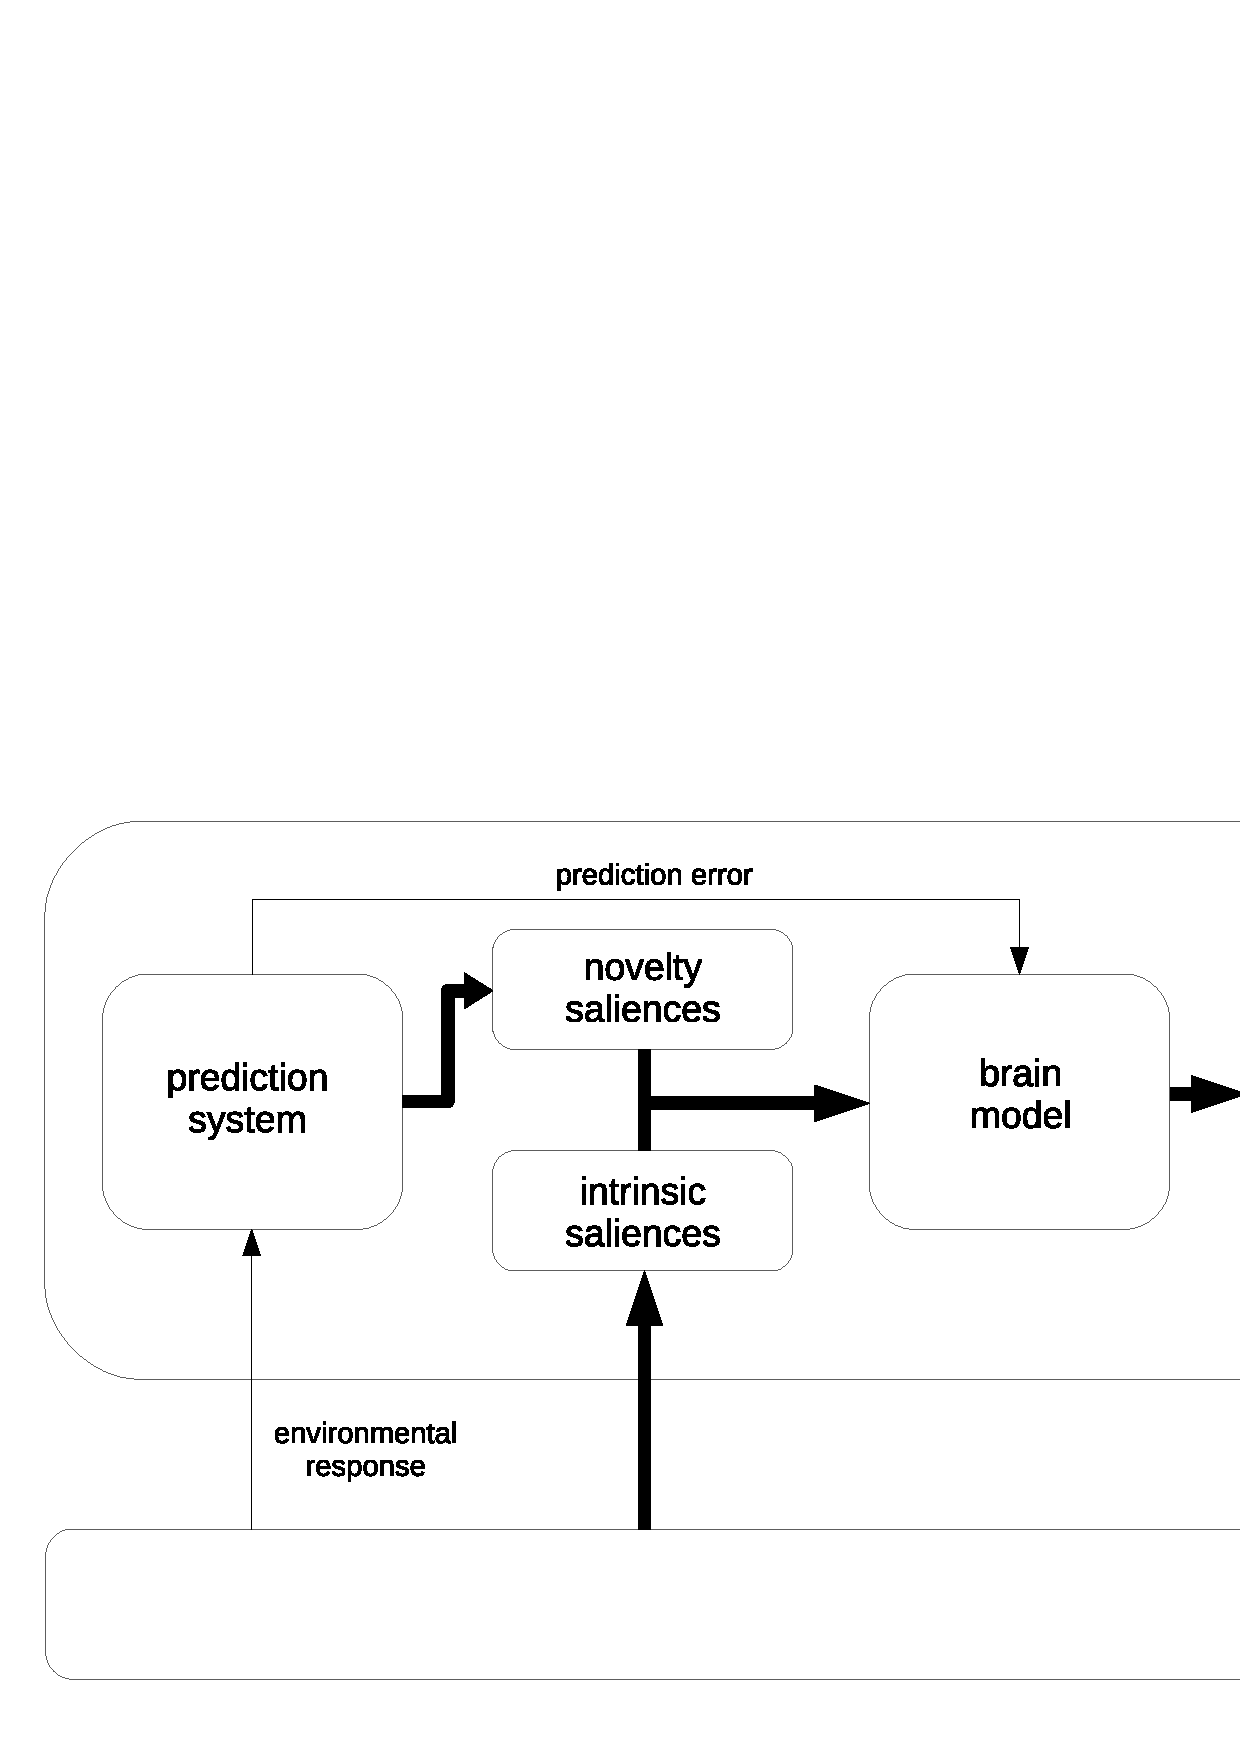
\includegraphics[width=\linewidth]{figs/model_schematic/model_schematic1.jpg}
\caption{Schematic of Model~1. The prediction system stores and processes the internal beliefs about the environment's behavior. It assigns to each possible action a novelty salience, which is combined with intrinsic salience and fed into the neural circuit model. Depending on its output, the current action is chosen and executed. Based on the environment's response, the prediction system is updated and the next iteration begins. Thin arrows denote propagation of scalar values, thick arrows indicate information flow within each parallel action channel.}
\label{fig:model1}
\end{figure}


\subsection{The Prediction System}
\label{sec:pred_system}

\subsubsection{Prediction Adaptation}
\label{sec:pred_adaptation}

The prediction system represents the agent's knowledge about the behavior of the environment. Specifically, it generates predictions about future sensory states following specific actions and captures learning by adapting internal belief variables (see Fig.~\ref{fig:prediction}A):
Let $y(t)$ be a scalar sensory feature at time $t$ and $y^*(t)$ its prediction. Then prediction adaptation follows
\begin{align}
y^*(t+\delta t) = y(t) - \tau_p \bigl(y(t) - y^*(t)\bigr),
\end{align}
where $\tau_p$ is the prediction adaptation time constant with $0<\tau_p<1$ and $\delta t=0.01$~seconds is one time step.

\begin{figure}
\centering
\includegraphics[width=4in]{figs/bolado-gomez13_fig5_3.pdf}
\caption{Processing within the prediction system. \textbf{(A)} Cartoon of a prediction trajectory. Every time the considered action is executed (circles), the prediction variable is updated based on the sensory outcome (red bars).
\textbf{(B)} Mapping from prediction onto novelty salience. The binary entropy function indicates the expected information gain based on the prediction variable, so uncertain outcomes yield higher saliences. The function is scaled for model consistency.
\textbf{(C)} The novelty salience corresponding to the prediction variable in \textbf{(A)}. Based on the mapping function in \textbf{(B)}, this salience reflects the evolution of the expected information gain for this action.
\textbf{(D)} The sensory prediction error corresponding to the prediction variable in \textbf{(A)}.
Adapted from~\cite{bg13}.}
\label{fig:prediction}
\end{figure}

Here $y$ represents the appearance of an animal picture, so $y$ is binary. In this case, the prediction $y^*$ can be interpreted as the agent's estimated probability that an animal picture will appear, i.e.,~the degree of belief that this event will happen. Importantly, $y^*$ exists for each considered action, so the agent expects different outcomes after different actions. Specifically, the prediction system stores and updates four variables $y^*_i$ with action index $i$, one for each action. However, because only one action (fixate the functioning disc) generates a non-zero response $y$, only the corresponding prediction variable will evolve over time\footnote{This would be different for the yoked condition. However, that case can be ignored as I'm only modelling the active condition.}. Thus I refer to this specific prediction whenever I mention prediction adaptation in the following sections and will omit the action index.

All prediction variables are initialized at 0 based on the assumption that initially the subjects did not expect to trigger animal pictures by looking anywhere on the screen. Between test times T0 and T1, the prediction variables are retained, reflecting memory retention during the short break between these tests. However, the prediction variables at the beginning of T2 ($y^*_{2,b}$) are reduced compared to the end of T1 ($y^*_{1,e}$) to take into account forgetting during the seven days between these tests:
\begin{align}
y^*_{2,b} = k_{ret}\, y^*_{1,e},
\end{align}
where $k_{ret}$ is an individual memory retention factor with $0<k_{ret}<1$.


\subsubsection{Novelty Salience}

For each action, the prediction system maps the internal prediction $y^*$ onto the action's novelty salience $s_n$. In contrast to the action's intrinsic salience (see below), this novelty salience represents the top-down, experience- and knowledge-based factor of action selection.

Novelty saliences are calculated based on the assumption that actions with uncertain outcomes are more salient than actions with predictable outcomes. Therefore, the mapping function $s_n(y^*)$ has a maximum at $y^*=0.5$ (maximal uncertainty) and minima at $y^*=0$ and $y^*=1$ (minimal uncertainty). Based on these constraints, the original model assumed a piecewise linear dependence between novelty salience and prediction. I replaced this piecewise linear function by the binary entropy function, which is defined as the expected amount of information generated by a Bernoulli process with outcome probabilities $p$ and $1-p$ and random variable $X$ (see Fig.~\ref{fig:prediction}B):
\begin{align}
H_b(X) = -p \log_2 p - (1-p) \log_2 (1-p).
\end{align}
Here $X$ is the binary sensory state $y$, and $p$ is the agent's estimated outcome probability $y^*$. To retain the original scaling, a prefactor is added, resulting in:
\begin{align}
s_n(y^*) = -\frac{1}{2} \Bigl( y^*\log_2 y^* + (1-y^*)\log_2 (1-y^*)\Bigr).
\end{align}
Ultimately, the novelty salience reflects the expected information gain per action based on the agent's current beliefs. This approach to implement intrinsic motivation, i.e.,~intrinsic motivation based on information maximization, has been proposed by Schmidhuber and others~\cite{schmidhuber91,schmidhuber91b,moulin-frier13}.


\subsubsection{Sensory Prediction Error}

Apart from salience generation, the prediction system also generates prediction error signals (see Fig.~\ref{fig:prediction}D), which are directly fed into the neural circuit model. They represent dopaminergic signals, which have been implicated in prediction errors of rewards~\cite{schultz97} as well as of sensory events~\cite{redgrave08}. In the basal ganglia model, they affect synaptic learning in the cortico-striatal interface (see below).

The sensory prediction error $e$ is evaluated whenever an action has been executed and is given by:
\begin{align}
e(t) = y_i(t) - y^*_i(t),
\end{align}
where $i$ is the index of the executed action.


%one of the four complementary areas on the experiment screen: the functioning disc, the nonfunctioning disc, the image area, and the white background. 
%Sensory input is transformed into salience signals giving rise to activity in the cortical action channels. 
%The cortex feeds its activity into different nuclei of the basal ganglia. These nuclei process the cortical input within the so-called selection, control, and No-Go pathways, which determine the final motor output. 
%Learning takes place as adaptations of the prediction system as well as in cortico-striatal projections and thereby leads to behavioral action preferences. 
%
%Cortico-striatal learning is modulated by a sensory prediction system comprising novelty salience and prediction errors, which determine phasic dopamine release.
%The sensory prediction system tracks the outcome of each action and estimates for each action the probability that it will trigger the appearance of an animal picture. 
%The prediction system assigns to each action a novelty salience corresponding to the uncertainty of the action's outcome. Here I modified the original model, which assumed a piecewise linear mapping between prediction and novelty salience. 
%Instead, I use the Shannon entropy, which reflects the expected information gain given the estimated outcome probabilities.
%Additionally, the prediction system regulates the level of phasic dopamine, which signals the detection of unexpected events and modulates the plasticity of the cortico-striatal projections.
%
%The model contains seven parameters that were fitted to the individual subjects' gaze behavior: the \emph{exploration rate}, which governs the probability of fixating a random location instead of the most salient one; the \emph{learning speed}, i.e.,~the adaptation rate of the prediction system; and five parameters related to the subjective visual saliences and habituation of the stimuli. I fitted the model using Covariance Matrix Adaptation -- Evolution Strategy (CMA-ES)~\cite{hansen06} based on similarity between the individual subject's and the model's gaze pattern rates.


\subsection{Intrinsic Salience}
\label{sec:int_sal}

In contrast to novelty salience (see above), intrinsic salience summarizes the bottom-up, sensation-based aspects of action selection. For each action there is an intrinsic salience value $s_i$, which may change over time and determine the probability to execute this action in the absence of knowledge and expectations.

In the case of fixations, the intrinsic salience per action directly reflects the visual salience of the corresponding fixation area. Therefore, $s_i$ of the central image area has the same initial value as the white background, is set to a high value once an image is triggered and decreases linearly ($s_i(t+\delta t) = s_i(t) - k_{im}$) thereafter until $s_i$ of the background is reached after 17~seconds to simulate the decreasing image contrast while the image is fading out.

Additionally, habituation is taken into account by decreasing the intrinsic salience only of action $i$ whenever action $i$ has been executed: $s_i(t+\delta t) = \tau_h s_i(t)$ with habituation time constant $\tau_h < 1$. Between the tests at T0 and T1 the intrinsic salience values are retained, whereas they are reinitialized at the start of T2 based on the assumption that the subjects dishabituate during the week-long break between T1 and T2 but not during the short break between T0 and T1.

Finally, the intrinsic saliences are added to the corresponding novelty saliences and fed into the neural circuit model.



\subsection{The Neural Circuit Model}
\label{sec:neural_circuit}

\subsubsection{Structure and Dynamics}

The neural circuit model incorporates a set of parallel neural networks (channels) representing processing loops through cortex, thalamus, basal ganglia, and brainstem. Each channel corresponds to one action.%In reference to the gaze-contingent learning task, I defined the actions as fixations within one of four complementary screen regions: the functioning disc, the nonfunctioning disc, the central image area, and the white background. Thus my model adaptation contains four action channels.

The network units represent neuron populations, which process the saliences of the corresponding action. They are instantiated by leaky integrator units, whose activation variable $a$ follows:
\begin{align}
\tau_m\frac{da}{dt} = -a(t)+I(t).
\end{align}
Here $\tau_m$ is the characteristic membrane time constant (40~ms), and $I$ is the summed, weighted input.

The corresponding normalized firing rate $r$ is computed using a piecewise linear squashing function with threshold $\epsilon$:
\begin{align}
r(a) = 
\begin{cases}
0 & a \le \epsilon\\
a-\epsilon & \epsilon < a \le 1+\epsilon\\
1 & a > 1+\epsilon.
\end{cases}
\end{align}

\begin{figure}
\centering
\includegraphics[width=\linewidth]{figs/bolado-gomez13_fig6.jpg}
\caption{\textbf{(A)} Schematic of the overall neural circuit model indicating the sensory and motor cortex, the thalamic system comprising the thalamic reticular nucleus (TRN) and the ventrolateral thalamus (VL), and the basal ganglia and brainstem. Each connection here includes four parallel action channels. \textbf{(B)} Schematic of the basal ganglia network model indicating subthalamic nucleus (STN), globus pallidus internal and external segment (GPi and GPe), substantia nigra pars reticulata and pars compacta (SNr and SNc). Compartments represent action channels with population activity level (gray bars). Note that four action channels are present in my model implementation. Adapted from~\cite{bg13}.}
\label{fig:network}
\end{figure}

Overall, the network model has a feedforward structure: input signals arrive in the cortex and ultimately lead to motor output via the brainstem (see Fig.~\ref{fig:network}). The salience generators activate cortical units. These units excite the basal ganglia via cortico-striatal projections onto both neuron populations expressing dopamine receptor type~1 (D1-striatum) and those expressing dopamine receptor type~2 (D2-striatum). These cortico-striatal projections are subject to dopamine-dependent synaptic plasticity (see below). The cortex also excites the subthalamic nucleus (STN), which sums its input across channels and excites both the external and internal segments of the globus pallidus (GPe and GPi) as well as the substantia nigra pars reticulata (SNr). In line with the focusing model of action selection~\cite{kandel_basalganglia}, the D1-striatum and D2-striatum form inhibitory pathways that converge onto the output nuclei, i.e.,~the GPi and SNr. Activity in the D1-striatum leads to selection of a specific action whereas activity in the D2-striatum inhibits the other action channels. Finally, the GPi and SNr project onto the thalamus and brainstem, where the final selection and execution of the action takes place.

\subsubsection{Synaptic Learning}

The cortico-striatal projections are the only plastic connections in the model and receive modulatory dopamine signals from the substantia nigra pars compacta (SNc), whose activity is determined by the prediction system (see Section~\ref{sec:pred_system}). The learning rule implemented in the cortico-striatal weights is derived from Gurney's dopamine-dependent plasticity rule, which is based on biological data~\cite{shen08}. In terms of rate-coded neurons, the expected weight change $\langle dw / dt \rangle$ takes the form:
\begin{align}
\Bigl\langle \frac{dw}{dt}\Bigr\rangle &= A_3 \tau^+ \tau^y y(y-\theta_{BCM}) x\\
\theta_{BCM} &= \langle y^2 \rangle C_{BCM} \\
C_{BCM} &= \frac{-(A_-^{D1/D2} \tau^- + A_+^{D1/D2} \tau^+)}{A_3 \tau^+ \tau^y}
\end{align}
where $x$ and $y$ are the pre- and postsynaptic firing rates, $\tau^+$ and $\tau^-$ time constants associated with post-pre and pre-post firing, $\tau_y$ a time constant associated with spike triplets, $A_3$ a plasticity factor for triplet timing, and $A_+^{D1/D2}$ and $A_-^{D1/D2}$ factors associated with post-pre and pre-post firing for D1-type and D2-type striatal neurons, respectively.

%\sloppy
The dopamine dependence is incorporated in the $A_+^{D1/D2}$ and $A_+^{D1/D2}$ factors. These factors were fitted to \emph{in vitro} data~\cite{shen08} using plasticity coefficients $A_{\pm}^{D1/D2 (\text{hi})}$ and $A_{\pm}^{D1/D2 (\text{lo})}$ signifying extreme ("high" and "low") levels of dopamine~\cite{gurney09}. Values for intermediate levels of dopamine $d$ are interpolated by a blending function $\alpha(d)$:
\begin{align}
\alpha(d) = \frac{4d}{1+4d}.
\end{align}
For instance, the dopamine-dependent contribution of positive spike pair timing in D1-type neurons is given by
\begin{align}
A_+^{D1}(d) = \alpha(d)A_+^{D1(\text{hi})}+(1-\alpha(d))A_+^{D1(\text{lo})}.
\end{align}
The factors $A_-^{D1}(d)$, $A_+^{D2}(d)$, and $A_-^{D2}(d)$ are defined similarly.

Finally, the plastic weights are modified according to
\begin{align}
w(t+\Delta t) = w(t) + \eta \Bigl\langle \frac{dw}{dt} \Bigr\rangle \Delta t,
\end{align}
where $\eta$ is the synaptic learning rate.



\subsection{Action Selection}

Action selection is implemented in a stochastic fashion to allow for exploratory behavior. Based on the output activities $r_{o,i}$ of the neural circuit model, the action probability distribution $p(i)$ is calculated using a softmax function:
\begin{align}
p(i) = \frac{\exp\Bigl(\frac{r_{o,i}}{k_{\text{exp}}}\Bigr)}{\sum_j \exp\Bigl(\frac{r_{o,j}}{k_{\text{exp}}}\Bigr)},
\end{align}
where $i$ is the action index and $k_{\text{exp}}>0$ is the individual exploration rate. The action is selected by sampling from this probability distribution.


\subsection{Environment}

The environment model simulates the experiment itself, i.e.,~the responses of the environment to each of the subject's action. Because only fixations on the functioning disc trigger a response, $y=0$ whenever another area is fixated. Taking into account the finite failure probabilities $p_f$ of the eye tracking system (see Section~\ref{sec:met_processing}), $y=0$ with probability $p_f$ and $y=1$ with probability $1-p_f$ after each fixation on the functioning disc. Also, successful image triggers modify the intrinsic salience of the central image area (see Section~\ref{sec:int_sal}).



\subsection{Parameter and Simulation Details}
\label{ssec:params}

The parameters listed in Table~\ref{tab:params_free1} are treated as free model paramters that are fitted to each subject (see Section~\ref{sec:model_fitting}). The parameter values listed in Tables~\ref{tab:params_network} and~\ref{tab:params_plasticity} are the original values used in~\cite{bg13}.

Simulated time steps cover 500~ms, which is about the average time period between fixations of the subjects. Simulations of each test were run until either 5 simulated minutes passed or 30 images were triggered by the agent.

\begin{center}
\begin{tabular}{ c  c }
\hline
Parameter & Description\\
\hline
$\tau_p$ & prediction adaptation time constant\\
$k_{\text{ret}}$ & memory retention factor\\
$\eta$ & synaptic learning rate\\
$k_{\text{exp}}$ & exploration rate\\
\hline
\end{tabular}
\captionof{table}{Free parameters subject to fitting.}
\label{tab:params_free1}
\end{center}


\begin{center}
\begin{tabular}{ c  c  c }
\hline
Parameter & Value & Description\\
\hline
$\tau_{h,\text{im}}$ & 0.81 & habituation time constant of central image area\\
$\tau_{h}$ & 0.77 & habituation time constant of other areas\\
$s_{i, \text{im}}$ & 0.49 & intrinsic salience of new animal picture\\
\hline
&& initial intrinsic salience of\\
$s_{i, L}(0)$ & 0.1 & left disc\\
$s_{i, R}(0)$ & 0.1 & right disc\\
$s_{i, W}(0)$ & 0.01 & white background\\
$s_{i, C}(0)$ & 0.01 & central image area\\
\hline
\end{tabular}
\captionof{table}{Parameters of intrinsic saliences.}
\label{tab:params_int_sal1}
\end{center}



\begin{center}
\begin{tabular}{ c  c  c }
\hline
Parameter & Value & Description\\
\hline
$\tau_m$ & 40 ms & membrane time constant\\
$\epsilon_S$ & 0 & sensory cortex activation threshold\\
$\epsilon_M$ & 0 & motor cortex activation threshold\\
$\epsilon_{TRN}$ & 0 & TRN activation threshold\\
$\epsilon_{VL}$ & 0 & VL activation threshold\\
$\epsilon_{BS}$ & 0 & brainstem activation threshold\\
$\epsilon_{D1}$ & 0.1 & D1 cells activation threshold\\
$\epsilon_{D2}$ & 0.1 & D2 cells activation threshold\\
$\epsilon_{STN}$ & -0.25 & STN activation threshold\\
$\epsilon_{GPe}$ & -0.2 & GPe activation threshold\\
$\epsilon_{GPi}$ & -0.075 & GPi activation threshold\\
$\epsilon_{SNc}$ & -0.198 & SNc activation threshold\\
$w_{S,M}$ & 1.0 & weight from sensory to motor cortex\\
$w_{VL,M}$ & 1.0 & weight from VL to motor cortex\\
$w_{M,TRN}$ & 1.0 & weight from motor cortex to TRN\\
$w_{VL,TRN}$ & 1.0 & weight from VL to TRN\\
$w_{M,VL}$ & 1.2 & weight from motor cortex to VL\\
$w_{GPi,VL}$ & 1.0 & weight from GPi to VL\\
$w_{TRN,VL}^w$ & 0.1 & weight from TRN to VL (within)\\
$w_{TRN,VL}^b$ & 0.3 & weight from TRN to VL (between)\\
$w_{S,D1/D2}^0$ & 0.5 & initial weights from sensory cortex to striatum\\
$w_{M,D1/D2}^0$ & 0.5 & initial weights from motor cortex to striatum\\
$w_{S,STN}$ & 0.3 & weight from sensory cortex to STN\\
$w_{M,STN}$ & 0.5 & weight from motor cortex to STN\\
$w_{GPe,STN}$ & 0.2 & weight from GPe to STN\\
$w_{STN,GPe}$ & 0.3 & weight from STN to GPe\\
$w_{D2,GPe}$ & 0.9 & weight from D2-striatum to GPe\\
$w_{STN,GPi}$ & 0.33 & weight from STN to GPi\\
$w_{D1,GPi}$ & 0.75 & weight from D1-striatum to GPi\\
$w_{GPe,GPi}$ & 0.4 & weight from GPe to GPi\\
$w_{SC, SNc}$ & 4.0 & weight from SC to SNc\\
$w_{M,BS}$ & 1.0 & weight from motor cortex to brainstem\\
$w_{GPi,BS}^+$ & 0.7 & additive weight from GPi to brainstem\\
$w_{GPi,BS}^x$ & 2.0 & multiplicative weight from GPi to brainstem\\
\hline
\end{tabular}
\captionof{table}{Parameters of the neural circuit model.}
\label{tab:params_network}
\end{center}

\begin{center}
\begin{tabular}{ c  c  c}
\hline
Parameter & Value & Description\\
\hline
$\tau^+$ & 38 ms & time constant for positive spike pair timing\\
$\tau^-$ & 38 ms & time constant for negative spike pair timing\\
$\tau^y$ & 45 ms & time constant for spike triplets\\
\hline
&& plasticity coefficients for\\
$A_3$ & 0.1 & spike triplets\\
$A_+^{D1(\text{lo})}$ & -0.2 & positive spike pair timing, D1-striatum, low dopamine level\\
$A_+^{D1(\text{hi})}$ & 1.27 & positive spike pair timing, D1-striatum, high dopamine level\\
$A_-^{D1(\text{lo})}$ & -0.8 & negative spike pair timing, D1-striatum, low dopamine level\\
$A_-^{D1(\text{hi})}$ & -0.15 & negative spike pair timing, D1-striatum, high dopamine level\\
$A_+^{D2(\text{lo})}$ & 0.4 & positive spike pair timing, D2-striatum, low dopamine level\\
$A_+^{D2(\text{hi})}$ & 0.25 & positive spike pair timing, D2-striatum, high dopamine level\\
$A_-^{D2(\text{lo})}$ & 0.3 & negative spike pair timing, D2-striatum, low dopamine level\\
$A_-^{D2(\text{hi})}$ & -1.5 & negative spike pair timing, D2-striatum, high dopamine level\\
\hline
\end{tabular}
\captionof{table}{Parameters of the cortico-striatal plasticity.}
\label{tab:params_plasticity}
\end{center}



\section{Model 2}
\label{sec:met_model2}

Model~2 is a simplified version of Model~1 (see Fig.~\ref{fig:model2}). It lacks the neural circuit model and is therefore less biologically realistic but more focussed on the functionality of prediction adaptation.

Action selection in Model~2 depends on the summed novelty and intrinsic saliences instead of the neural circuit model output.
The used parameter values are listed in Table~\ref{tab:params_int_sal2}. All other parts of Model~2 are identical to Model~1.


\begin{figure}
\centering
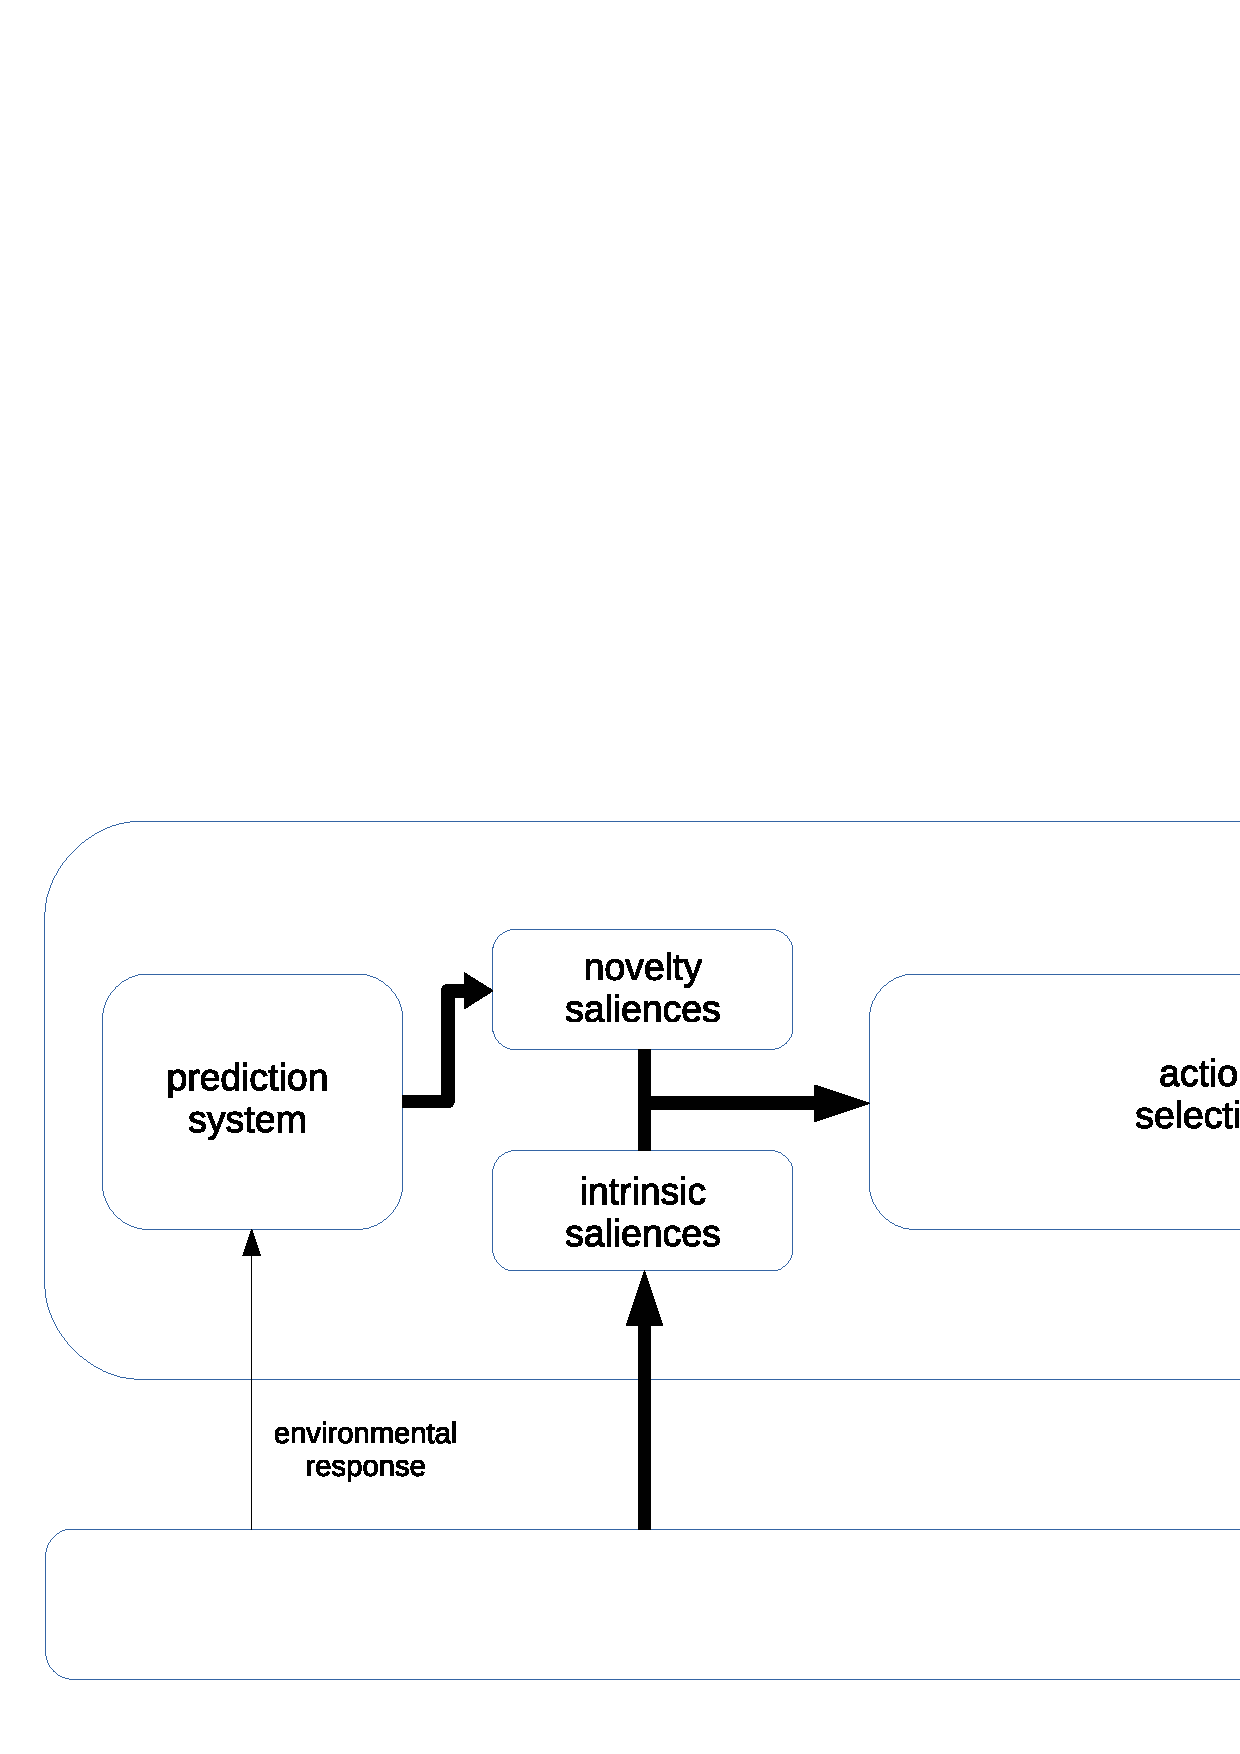
\includegraphics[width=\linewidth]{figs/model_schematic/model_schematic2.jpg}
\caption{Schematic of Model~2, which is essentially Model~1 without the neural circuit model (see Fig.~\ref{fig:model1}, same conventions).}
\label{fig:model2}
\end{figure}

\begin{center}
\begin{tabular}{ c  c }
\hline
Parameter & Description\\
\hline
$\tau_p$ & prediction adaptation time constant\\
$k_{\text{ret}}$ & memory retention factor\\
$k_{\text{exp}}$ & exploration rate\\
\hline
\end{tabular}
\captionof{table}{Free parameters subject to fitting.}
\label{tab:params_free2}
\end{center}


\begin{center}
\begin{tabular}{ c  c  c }
\hline
Parameter & Value & Description\\
\hline
$s_{i, L}(0)$ & 0.1 & initial intrinsic salience of left disc\\
$s_{i, R}(0)$ & 0.1 & initial intrinsic salience of right disc\\
$s_{i, W}(0)$ & 0.01 & initial intrinsic salience of white background\\
$s_{i, C}(0)$ & 0.01 & initial intrinsic salience of central image area\\
$s_{i, \text{im}}$ & 0.5 & intrinsic salience of new animal picture\\
$\tau_{h}$ & 0.8 & habituation time constant of all areas\\
\hline
\end{tabular}
\captionof{table}{Parameters of intrinsic saliences.}
\label{tab:params_int_sal2}
\end{center}


\section{Model Fitting}
\label{sec:model_fitting}

For both models, the free parameters were fitted to each subject using Covariance Matrix Adaptation--Evolution Strategy (CMA-ES)~\cite{hansen06}, a stochastic optimization algorithm.

Each sampled set of parameters was evaluated by simulating the model and extracting the bias (see Section~\ref{sec:bias}) from the simulated agent's behavior during the three tests. The sample's fitness error $f$ was then:
\begin{align}
f &= \sum^2_{T=0} c_T \, (b^{\text{exp}}_{T} - b^{\text{sim}}_{T})^2 \\
c_T &= 
\begin{cases}
0 & \text{ if failure rate $>$ 0.1 during test $T$,}\\
1 & \text{ else,}
\end{cases}
\end{align}
where $b^{\text{exp}}_T$ is the empirical bias of the subject during test $T$, i.e., the bias extracted from the experimental data, and $b^{\text{sim}}_T$ the simulated agent's bias during test $T$, i.e., the bias extracted from the simulation data.

The fitting was terminated as soon as the best sample's fitness error fell below 0.1 times the number of tests with a failure rate of at most 0.1. This sample's parameters were then accepted as the fitting results for that subject. Otherwise, if the parameters or fitness error converged, or the conditioning number of the covariance matrix diverged, the parameters were reset and the step sized increased by 0.05 up to a maximum of 0.5. After 100 search reinitializations the best set of parameters was selected as the fitting solution.

The sampling parameters are listed in Table~\ref{tab:params_sampling}. The population size $\lambda$ was 99, and the other hyperparameters were set as recommended in~\cite{hansen11}.

\begin{center}
\begin{tabular}{ c  c  c  c }
\hline
Parameter & Initial Value & Standard Deviation & Description\\
\hline
$\tau_{p}$ & 0.9 & 0.05 & prediction adaptation time constant\\
$k_{\text{ret}}$ & 0.9 & 0.1 & memory retention factor\\
$\eta$ & 100 & 10 & synaptic learning rate\\
&&& (only Model~1)\\
$k_{\text{exp}}$ & 0.6 & 0.1 & exploration rate\\
\hline
\end{tabular}
\captionof{table}{Sampling parameters during fitting.}
\label{tab:params_sampling}
\end{center}







\chapter{Results}
\label{ch:results}


\subsubsection{Conventions}

In this chapter's figures, samples are indicated by their means. Error bars indicate the standard errors of the means. In case of box plots, horizontal lines in boxes indicate first quartile, median, and third quartile. Whiskers cover the range of the data up to 1.5 times the interquartile range. Crosses indicate extreme outliers. The mean is marked by squares.

Unless stated otherwise, deviations of sample means are tested using Student's t-test. Significant deviations are graphically indicated by * ($p<0.05$), ** ($p<0.01$), or *** ($p<0.001$). Significant deviations between two samples are indicated by bars. Asterisks without bars indicate a significant deviation of the sample mean from 0.

In case of correlation analysis, the following measures are reported:
\begin{itemize}
\item the adjusted $R^2$ of the regression,
\item the Pearson coefficient of correlation,
\item the p-value of a correlation t-test,
\item the adjusted p-value using the Holm-Bonferroni method~\cite{holm79}.
\end{itemize}
The regression line is plotted along with the corresponding 95\% confidence bands.

Outliers of a given sample are defined as all data points lying outside of range
\begin{align}
\Bigl[\text{Q1} - 1.5 \cdot \text{IQR}, \text{Q3} + 1.5 \cdot \text{IQR}\Bigr],
\end{align}
where IQR $=$ Q3 $-$ Q1 is the sample's interquartile range, and Q1 and Q3 are its first and third quartile, respectively.



\section{Behavioral Bias}
\label{sec:bias}

A first qualitative assessment of the subjects' gaze behaviors revealed a higher concentration of fixations on the functioning disc than on the non-functioning one during the active control sessions (see Fig.~\ref{fig:fix_dist}a), indicating a preference for the functioning over the non-functioning disc. During the yoked control sessions, no such preference was observed (see Fig.~\ref{fig:fix_dist}b), which implies that the behavioral bias is indeed tied to the functionality of the functioning disc.

\begin{figure}
\centering
    \begin{subfigure}[b]{0.49\textwidth}
        \includegraphics[width=\textwidth]{figs/sec3/active_nofix_2.png}
        \caption{Gaze-Contingent Tests}
    \end{subfigure}
\begin{subfigure}[b]{0.49\textwidth}
        \includegraphics[width=\textwidth]{figs/sec3/yoked_nofix_2.png}
        \caption{Yoked Control Tests}
    \end{subfigure}
\caption{Aggregate fixation distribution during all gaze-contingent tests (a) and yoked control tests at T0 (b). The central rectangle indicates the location of the animal pictures, the circles the locations of the red discs. In (a), fixation locations during tests with the functioning disc on the left were mirrored along the central vertical axis such that the functioning disc is visualized on the right. The density estimation is described in Section~\ref{sec:met_processing}. Adapted from~\cite{kolling17}.}
\label{fig:fix_dist}
\end{figure}

To quantify this preference, I applied the notion of \textit{gaze patterns} as introduced in~\cite{wang12} and extended in~\cite{kolling17}: A (non-)functioning gaze pattern is defined as a fixation sequence starting in the central image area, leading to the (non-)functioning disc and back to the image area. Because the total experiment durations varied between subjects and tests, the gaze pattern counts were divided by the test durations to yield the normalized \textit{gaze pattern rates}~\cite{kolling17}. To take into account the different activity levels of subjects, I finally define the \textit{functioning bias} as the difference between the functioning gaze pattern rate and the non-functioning gaze pattern rate. This scalar quantity is plotted in units~$\frac{1}{\text{min}}$ and indicates whether a subject preferred the functioning disc (bias $>0$), the non-functioning disc (bias $<0$), or showed no preference (bias $\approx 0$). Thus for all bias samples, the deviations from 0 are analyzed.

The experimental data indicate that the subjects\footnote{Only gaze-contingent tests are considered henceforth.} prefer the functioning disc at T0 and tend to increase this preference during repeated tests (see Fig.~\ref{fig:bias}a). This functioning bias is highly significant when averaged over all tests.

The models were fitted to these data (see Section~\ref{sec:model_fitting}).\footnote{Only individual subjects were fitted.} The model fits faithfully reproduce the experimental data (see Fig.~\ref{fig:bias}b). Figure~\ref{fig:bias}c shows the empirical functioning bias as well as the model fits including their estimations for the tests that were excluded from the analysis because of the failure rate estimation (see sections~\ref{sec:met_experiment} and~\ref{sec:met_processing}). Both models estimate a slightly higher bias during T0 for subjects missing in the empirical T0 data, which implies a systematic trend: If a subject would exhibit a high bias, his T0 test is more likely to be rejected due to its failure rate than for a subject with low bias, according to the models. Why this should be so is unclear. These model estimates (or predictions) are the basis for the following analyses. 

Note that estimating the retention factor is problematic in cases where T2 data are not present. In this case, the fitting algorithm would be able to estimate an arbitrary value for the retention factor. However, in practice it estimates a value around the initial search value (see Table~\ref{tab:params_sampling}). Due to these difficulties, I disregard the estimated retention in the following analyses.

Histograms of the achieved fitness errors are plotted in Figure~\ref{fig:fitness}.

\begin{figure}
\centering
    \begin{subfigure}[b]{0.49\textwidth}
\includegraphics[width=\textwidth]{figs/sec3/bias_all_dat.jpeg}
\caption{Experiment}
    \end{subfigure}
    
    \begin{subfigure}[b]{0.49\textwidth}
        \includegraphics[width=\textwidth]{figs/sec3/fitting/fitting_reduced.jpeg}
        \caption{Model Fits}
    \end{subfigure}
\begin{subfigure}[b]{0.49\textwidth}
        \includegraphics[width=\textwidth]{figs/sec3/fitting/fitting_all.jpeg}
        \caption{Full Simulation Data}
    \end{subfigure}
\caption{(a) Functioning bias of all subjects tested in the gaze-contingent condition. (b)~Experimental data and their model fits. (c) Experimental and full simulation data.}
\label{fig:bias}
\end{figure}

\begin{figure}
\centering
    \begin{subfigure}[b]{0.49\textwidth}
        \includegraphics[width=\textwidth]{figs/sec3/fitting/fitness_mod1.jpeg}
        \caption{Model 1}
    \end{subfigure}
\begin{subfigure}[b]{0.49\textwidth}
        \includegraphics[width=\textwidth]{figs/sec3/fitting/fitness_mod2.jpeg}
        \caption{Model 2}
    \end{subfigure}
\caption{Histograms of subjects' fitness errors for model 1 (a) and model 2 (b).}
\label{fig:fitness}
\end{figure}

\clearpage

\section{Effect of Age}
\label{sec:age}

Analysing the behavior of different age groups reveals that this functioning bias is mostly due to the 8-month-old subjects, who show a consistent bias during all tests (see Fig.~\ref{fig:age_diff_dat}). The 6-month-olds don't show a bias during any test, whereas the 10-month-olds do during T2 and when averaged over tests. 
Both models estimate a similarly biased behavior of the 8- and 10-month-old subjects and a functioning bias of the 6-month-olds when averaged over tests (see Figs.~\ref{fig:age_diff_mod1} and~\ref{fig:age_diff_mod2}).

\begin{figure}
\centering
    \begin{subfigure}[b]{0.49\textwidth}
        \includegraphics[width=\textwidth]{figs/sec3/age/age_diff1_dat.jpeg}
        \caption{T0}
    \end{subfigure}
\begin{subfigure}[b]{0.49\textwidth}
        \includegraphics[width=\textwidth]{figs/sec3/age/age_diff2_dat.jpeg}
        \caption{T1}
    \end{subfigure}
    
    \begin{subfigure}[b]{0.49\textwidth}
        \includegraphics[width=\textwidth]{figs/sec3/age/age_diff3_dat.jpeg}
        \caption{T2}
    \end{subfigure}
    \begin{subfigure}[b]{0.49\textwidth}
        \includegraphics[width=\textwidth]{figs/sec3/age/age_diff_mean_dat.jpeg}
        \caption{Average Over Tests}
    \end{subfigure}
\caption{Empirical functioning bias of different age groups during individual tests (a-c) and averaged over tests (d). Dashed lines indicate level of unbiased behavior.}
\label{fig:age_diff_dat}
\end{figure}

\begin{figure}
\centering
    \begin{subfigure}[b]{0.49\textwidth}
        \includegraphics[width=\textwidth]{figs/sec3/age/age_diff1_mod1.jpeg}
        \caption{T0}
    \end{subfigure}
\begin{subfigure}[b]{0.49\textwidth}
        \includegraphics[width=\textwidth]{figs/sec3/age/age_diff2_mod1.jpeg}
        \caption{T1}
    \end{subfigure}
    
    \begin{subfigure}[b]{0.49\textwidth}
        \includegraphics[width=\textwidth]{figs/sec3/age/age_diff3_mod1.jpeg}
        \caption{T2}
    \end{subfigure}
    \begin{subfigure}[b]{0.49\textwidth}
        \includegraphics[width=\textwidth]{figs/sec3/age/age_diff_mean_mod1.jpeg}
        \caption{Average Over Tests}
    \end{subfigure}
\caption{Functioning bias of different age groups during individual tests (a-c) and averaged over tests (d) as estimated by model 1. Dashed lines indicate level of unbiased behavior.}
\label{fig:age_diff_mod1}
\end{figure}

\begin{figure}
\centering
    \begin{subfigure}[b]{0.49\textwidth}
        \includegraphics[width=\textwidth]{figs/sec3/age/age_diff1_mod2.jpeg}
        \caption{T0}
    \end{subfigure}
\begin{subfigure}[b]{0.49\textwidth}
        \includegraphics[width=\textwidth]{figs/sec3/age/age_diff2_mod2.jpeg}
        \caption{T1}
    \end{subfigure}
    
    \begin{subfigure}[b]{0.49\textwidth}
        \includegraphics[width=\textwidth]{figs/sec3/age/age_diff3_mod2.jpeg}
        \caption{T2}
    \end{subfigure}
    \begin{subfigure}[b]{0.49\textwidth}
        \includegraphics[width=\textwidth]{figs/sec3/age/age_diff_mean_mod2.jpeg}
        \caption{Average Over Tests}
    \end{subfigure}
\caption{Functioning bias of different age groups during individual tests (a-c) and averaged over tests (d) as estimated by model 2. Dashed lines indicate level of unbiased behavior.}
\label{fig:age_diff_mod2}
\end{figure}

To study this qualitative difference of the 6-month-olds on the one hand and the 8- and 10-month-olds on the other hand, I grouped the latter and compared the two resulting groups. Empirically, the 6-month-olds show no functioning bias, whereas the older subjects consistently prefer the functioning disc during all tests (see Fig.~\ref{fig:age2_diff_dat}). The behavior of the older subjects is reproduced by both models (see Figs.~\ref{fig:age2_diff_mod1} and~\ref{fig:age2_diff_mod2}). Both models agree on a significantly stronger bias of the older subjects compared to the 6-month-olds during T1. However, Model~1 estimates unbiased behavior of the 6-month-olds during T2 and a significantly lower one overall, whereas Model~2 estimates a similar bias level during T2 and overall. In summary, both models reproduce the consistent functioning bias exhibited by the older subjects. The models indicate that the difference is highest during T1 and predict that also the 6-month-olds show a functioning bias on average.

\begin{figure}
\centering
    \begin{subfigure}[b]{0.49\textwidth}
        \includegraphics[width=\textwidth]{figs/sec3/age/age2_diff1_dat.jpeg}
        \caption{T0}
    \end{subfigure}
\begin{subfigure}[b]{0.49\textwidth}
        \includegraphics[width=\textwidth]{figs/sec3/age/age2_diff2_dat.jpeg}
        \caption{T1}
    \end{subfigure}
    
    \begin{subfigure}[b]{0.49\textwidth}
        \includegraphics[width=\textwidth]{figs/sec3/age/age2_diff3_dat.jpeg}
        \caption{T2}
    \end{subfigure}
    \begin{subfigure}[b]{0.49\textwidth}
        \includegraphics[width=\textwidth]{figs/sec3/age/age2_diff_mean_dat.jpeg}
        \caption{Average Over Tests}
    \end{subfigure}
\caption{Empirical functioning bias of different age groups during individual tests (a-c) and averaged over tests (d). Dashed lines indicate level of unbiased behavior.}
\label{fig:age2_diff_dat}
\end{figure}

\begin{figure}
\centering
    \begin{subfigure}[b]{0.49\textwidth}
        \includegraphics[width=\textwidth]{figs/sec3/age/age2_diff1_mod1.jpeg}
        \caption{T0}
    \end{subfigure}
\begin{subfigure}[b]{0.49\textwidth}
        \includegraphics[width=\textwidth]{figs/sec3/age/age2_diff2_mod1.jpeg}
        \caption{T1}
    \end{subfigure}
    
    \begin{subfigure}[b]{0.49\textwidth}
        \includegraphics[width=\textwidth]{figs/sec3/age/age2_diff3_mod1.jpeg}
        \caption{T2}
    \end{subfigure}
    \begin{subfigure}[b]{0.49\textwidth}
        \includegraphics[width=\textwidth]{figs/sec3/age/age2_diff_mean_mod1.jpeg}
        \caption{Average Over Tests}
    \end{subfigure}
\caption{Functioning bias of different age groups during individual tests (a-c) and averaged over tests (d) as estimated by model 1. Dashed lines indicate level of unbiased behavior.}
\label{fig:age2_diff_mod1}
\end{figure}

\begin{figure}
\centering
    \begin{subfigure}[b]{0.49\textwidth}
        \includegraphics[width=\textwidth]{figs/sec3/age/age2_diff1_mod2.jpeg}
        \caption{T0}
    \end{subfigure}
\begin{subfigure}[b]{0.49\textwidth}
        \includegraphics[width=\textwidth]{figs/sec3/age/age2_diff2_mod2.jpeg}
        \caption{T1}
    \end{subfigure}
    
    \begin{subfigure}[b]{0.49\textwidth}
        \includegraphics[width=\textwidth]{figs/sec3/age/age2_diff3_mod2.jpeg}
        \caption{T2}
    \end{subfigure}
    \begin{subfigure}[b]{0.49\textwidth}
        \includegraphics[width=\textwidth]{figs/sec3/age/age2_diff_mean_mod2.jpeg}
        \caption{Average Over Tests}
    \end{subfigure}
\caption{Functioning bias of different age groups during individual tests (a-c) and averaged over tests (d) as estimated by model 2. Dashed lines indicate level of unbiased behavior.}
\label{fig:age2_diff_mod2}
\end{figure}

Differences in simulated behavior should be reflected in the underlying model parameters. Even though slight differences in the fitted parameters exist, none of them are significant (see Figs.~\ref{fig:age2_params1} and~\ref{fig:age2_params2}).

\begin{figure}
\centering
    \begin{subfigure}[b]{0.49\textwidth}
        \includegraphics[width=\textwidth]{figs/sec3/age/age2_pred_mod1.jpeg}
        \caption{Model 1}
    \end{subfigure}
\begin{subfigure}[b]{0.49\textwidth}
        \includegraphics[width=\textwidth]{figs/sec3/age/age2_pred_mod2.jpeg}
        \caption{Model 2}
    \end{subfigure}
    
    \begin{subfigure}[b]{0.49\textwidth}
        \includegraphics[width=\textwidth]{figs/sec3/age/age2_ret_mod1.jpeg}
        \caption{Model 1}
    \end{subfigure}
    \begin{subfigure}[b]{0.49\textwidth}
        \includegraphics[width=\textwidth]{figs/sec3/age/age2_ret_mod2.jpeg}
        \caption{Model 2}
    \end{subfigure}
    
        \begin{subfigure}[b]{0.49\textwidth}
        \includegraphics[width=\textwidth]{figs/sec3/age/age2_temp_mod1.jpeg}
        \caption{Model 1}
    \end{subfigure}
\begin{subfigure}[b]{0.49\textwidth}
        \includegraphics[width=\textwidth]{figs/sec3/age/age2_temp_mod2.jpeg}
        \caption{Model 2}
    \end{subfigure}
\caption{Distributions of the fitted parameters $\tau_p$ (a,b), $k_{ret}$ (c,d), and $k_{exp}$ (e,f) for 6-month-olds and older subjects.}
\label{fig:age2_params1}
\end{figure}

\begin{figure}
\centering        
\includegraphics[width=0.5\textwidth]{figs/sec3/age/age2_sigma_lr_mod1.jpeg}
\caption{Distributions of the fitted synaptic learning rate $\eta$  for 6-month-olds and older subjects. This parameter is not present in Model~2.}
\label{fig:age2_params2}
\end{figure}

Let us turn to studying the functioning bias on the level of individual subjects, which promises deeper insights.

\clearpage

\section{Individual Learning Progress}
\label{sec:ind_learning}

The main hypothesis of this study is that subjects acquire the gaze-contingency during the experiments, i.e.,~they learn to predict the appearance of an animal picture after they fixate the functioning disc. This process is modelled by adaptation of the prediction system. Specifically, the prediction variable $y^*$ converges to 1 during learning (see Section~\ref{sec:pred_adaptation}). The more uncertain the agent is about the outcome of the action, i.e.,~the closer $y^*$ is to 0.5, the higher its associated novelty salience and thus the higher the probability of performing that action. So the resulting behavioral bias is based on the transition of the internal prediction through the uncertain regime ($y^*$~around 0.5) as indicated by the magnitude of the novelty salience.

Figure~\ref{fig:learners_pred} shows the time evolution of the predictions and the corresponding novelty saliences for three simulated subjects representing three types of learning dynamics:
\begin{itemize}
\item The \textit{fast learner} (see Fig.~\ref{fig:learners_pred}a) quickly acquires the contingency within the first session, as indicated by the rapid convergence of $y^*$ to 1. As a result, the novelty salience quickly rises and falls in the beginning of the first session. The subject's internal model is fully adapted by the time session~2 starts, which is why no learning progress takes place and novelty salience is negligible during session~2. Depending on the memory retention factor, the subject may forget the contingency between T1 and T2, i.e.,~$y^*$ drops after T1 and quickly rises again during T2. During this readaptation, the novelty salience may peak again and result in another period of biased behavior.
\item The \textit{slow learner's} prediction (see Fig.~\ref{fig:learners_pred}b) evolves similarly, but on a longer time scale. During T0, $y^*$ is mostly in the uncertain regime, yielding a high level of novelty salience. The contingency is acquired by the end of the second session, which is still largely affected by the slowly decreasing novelty salience. Forgetting between T1 and T2 may again lead to a similar picture during T2 as during T0. In the end, high levels of novelty salience strongly bias the subject's behavior during all sessions, especially during T0 and T2.
\item The \textit{non-learner} (see Fig.~\ref{fig:learners_pred}c) steadily improves his prediction throughout the sessions but fails to acquire the contingency due to the slow rate of prediction adaptation. Because $y^*$ lies in the uncertain regime for most of the experiments, a high level of novelty salience is quickly reached during T0 and retained for the rest of the sessions, which results in a strong, persistent bias from early on.
\end{itemize}

\begin{figure}
\centering
    \begin{subfigure}[b]{0.49\textwidth}
        \includegraphics[width=\textwidth]{figs/sec3/fastlearner_mod1.jpeg}
        \caption{Fast Learner}
    \end{subfigure}
\begin{subfigure}[b]{0.49\textwidth}
        \includegraphics[width=\textwidth]{figs/sec3/slowlearner_mod1.jpeg}
        \caption{Slow Learner}
    \end{subfigure}
    
    \begin{subfigure}[b]{0.49\textwidth}
        \includegraphics[width=\textwidth]{figs/sec3/nonlearner_mod1.jpeg}
        \caption{Non-Learner}
    \end{subfigure}
\caption{Time evolution of the prediction variable $y^*$ (black) and the corresponding novelty salience (red) during simulated experiments for three individual subjects. Vertical dashed lines indicate session onsets. Note that a decrease of $y^*$ is either due to forgetting between T1 and T2 or due to trigger failures (see Section~\ref{sec:met_processing}), which contradict the contingency and lead to transient reversals of the prediction adaptation.}
\label{fig:learners_pred}
\end{figure}

Confirming these arguments, both models reproduce and offer explanations for the different levels of bias observed during these subjects' sessions and estimate the bias during the missing sessions (see Fig.~\ref{fig:learners_bias}). Note that I chose these three subjects because they represent extreme cases of different predicted learning dynamics and thereby serve as illustrative examples of different types of model behavior. Considering that in fewer than 10\% of all cases, subjects performed all three tests with failure rate less than 10\% (see Table~\ref{tab:filtered_groups}), it is not likely to find good examples only within subjects with all three tests remaining in the analysis. It is not required since we are focussing on the model behavior at this point.

Both models estimate the same qualitative behavior for these subjects during the missing sessions, which indicates that the biological component of Model~1 does not have a large impact on the finally chosen action. Note the interesting behavior of the fast learner, who starts with an initial negative bias and then shows a positive bias at T1. As we have just observed, the fast learner is least influenced by novelty salience since acquisition is rapidly over. This implies that he is more influenced by intrinsic salience, which is subject to habituation, which in turn favors equal proportions of fixations on both discs. Since he starts with an excess of fixations on the non-functioning disc (as required by the experimental data), due to habituation its intrinsic salience is much lower at the start of T1 than the one of the functioning disc. This is why both models would agree on a functioning bias for the fast learner during T1. Ultimately, this is an effect due to habituation and this particular initial condition and not much related to learning itself.

\begin{figure}
\centering
\begin{subfigure}[b]{0.49\textwidth}
        \includegraphics[width=\textwidth]{figs/sec3/individuals_diff_dat.jpeg}
        \caption{Experiment}
    \end{subfigure}

        \begin{subfigure}[b]{0.49\textwidth}    
            \includegraphics[width=\textwidth]{figs/sec3/individuals_diff_mod1.jpeg}
        \caption{Model 1}
    \end{subfigure}    
    \begin{subfigure}[b]{0.49\textwidth}
        \includegraphics[width=\textwidth]{figs/sec3/individual_diff_mod2.jpeg}
        \caption{Model 2}
    \end{subfigure}
\caption{Functioning bias of the subjects of Fig.~\ref{fig:learners_pred}: experimental data (a) and simulated behavior (b and c). Dashed lines indicate level of unbiased behavior.}
\label{fig:learners_bias}
\end{figure}

To quantify the speed with which each subject transitions through the uncertain regime and acquires the contingency, I introduce two measures, which are extracted from the subject's simulated predictions:
\begin{itemize}
\item \textit{t5}\footnote{Other fitting names for this quantity might be t0.5 or t50. However, I will stick with this notation for brevity's sake. The same holds for t9.} is the normalized experiment time at which $y^*$ first exceeds 0.5 (or 50\%). This is the moment of maximal uncertainty and thus maximal novelty salience.
\item \textit{t9} is the normalized experiment time at which $y^*$ first exceeds 0.9 (or 90\%). t9 indicates when a subject has reached a high confidence of predicting the contingent response. Because $y^*$ never reaches 1 (due to the exponential prediction adaptation, see Section~\ref{sec:pred_adaptation}), t9 may be interpreted as an approximation of the contingency acquisition time.
\end{itemize}

A time point's \textit{normalized experiment time} is computed by dividing its absolute simulated time by the session's duration, which allows to compare different sessions' time points on a relative scale. The normalized experiment time lies within $[0,3[$ with:
\begin{align}
\text{normalized experiment time} \in 
\begin{cases}
[0,1[ & \text{during T0,}\\
[1,2[ & \text{during T1,}\\
[2,3[ & \text{during T2.}
\end{cases}
\end{align}

Figure~\ref{fig:ind_preds} visualizes these measures for the fast learner, the slow learner, and the non-learner. In line with the previous discussion, the fast learner exhibits the smallest t5 whereas the non-learner exhibits the largest one. Additionally, the fast learner's t9 falls within T0 and the slow learner's t9 within T1, confirming the previously indicated times of contingency acquisition. Also, the non-learner's t9 is not defined since $y^*$ does not reach 0.9 during the sessions.

\begin{figure}
\centering        
\includegraphics[width=0.75\textwidth]{figs/sec3/individuals_preds.jpeg}
\caption{Prediction variables of Fig.~\ref{fig:learners_pred} plotted over normalized experiment time. Vertical dashed lines indicate session onsets. The green dashed line marks $y^*=0.5$; crossing this line for the first time defines a subject's t5. The purple dashed line marks $y^*=0.9$; crossing this line for the first time defines a subject's t9.}
\label{fig:ind_preds}
\end{figure}

The analysis of this chapter indicates that the adaptation rate of the internal prediction may be a key quantity determining the strength of the functioning bias. This idea is studied more closely in the next section.


\section{Learning Speed}
\label{sec:learning_speed}

\subsection{Median Split}
\label{sec:learning_speed_median_split}

To determine the effect of the prediction adaptation rate on the functioning bias within the whole sample, I first divided the subjects into two groups using a median split with respect to fitted prediction adaptation time constant $\tau_p$: Half of the subjects had below-median $\tau_p$ and formed the \textit{fast learners} group; the other half had above-median $\tau_p$ and formed the \textit{slow learners} group.
The resulting group bias is plotted in Figure~\ref{fig:pred_split}:
\begin{itemize}
\item Forming the fast and slow learners groups with respect to the Model~1 fits of $\tau_p$ yields the Model~1 estimates of the group bias (see Fig.~\ref{fig:pred_split}a). The model predicts a qualitatively different behavior of the two groups: While the slow learners exhibit a highly significant functioning bias throughout all sessions, the fast learners show unbiased behavior on average and during T0. While the bias approaches a similar level at T1, the slow learners' functioning bias is much higher during T0, T2, and on average. 
\item Considering the experimental data of the same subject groups exposes an even stronger discrepancy (see Fig.~\ref{fig:pred_split}b). The slow learners again exhibit a significant functioning bias throughout all sessions, confirming the model prediction. However, the fast learners show a consistently unbiased behavior throughout all sessions. The bias difference is significant during each session.
\item Conversely, forming the two groups with respect to the Model~2 fits of $\tau_p$ yields the Model~2 estimates of the group bias (see Fig.~\ref{fig:pred_split}c). Model~2 predicts a smaller difference between groups. Only the fast learners at T0 show unbiased behavior. On average, the slow learners exhibit a more biased behavior than the fast learners, which also holds for T0 only.
\item Again, the corresponding median split of the experimental data yields more pronounced differences than the model predicts (see Fig.~\ref{fig:pred_split}d). During all sessions, the slow learners exhibit a significant functioning bias whereas the fast learners do not. The differences are significant during T0, T2, and on average.
\end{itemize}

To summarize, the median split analyses of both models indicate that slow adaptation of the internal prediction leads to a pronounced behavioral bias whereas fast adaptation does less so or not at all.

\begin{figure}
\centering
\begin{subfigure}[b]{0.49\textwidth}
        \includegraphics[width=\textwidth]{figs/sec3/pred/pred_mod1mod1.jpeg}
        \caption{Model 1}
    \end{subfigure}
    \begin{subfigure}[b]{0.49\textwidth}
        \includegraphics[width=\textwidth]{figs/sec3/pred/pred_mod1dat.jpeg}
        \caption{Experiment}
    \end{subfigure}

\begin{subfigure}[b]{0.49\textwidth}
        \includegraphics[width=\textwidth]{figs/sec3/pred/pred_mod2mod2.jpeg}
        \caption{Model 2}
    \end{subfigure}
    \begin{subfigure}[b]{0.49\textwidth}
        \includegraphics[width=\textwidth]{figs/sec3/pred/pred_mod2dat.jpeg}
        \caption{Experiment}
    \end{subfigure}
\caption{Functioning bias of subject groups defined by median split of fitted $\tau_p$ based on Model~1 fits (a,b) and Model~2 fits (c,d). The groups' bias is plotted using the full simulation data (a,c) and the corresponding experimental data (b,d). The dashed lines indicate the level of unbiased behavior.}
\label{fig:pred_split}
\end{figure}


\subsection{Bias Correlations}
\label{sec:learning_speed_bias_correlations}

To further investigate the relation between the functioning bias and the speed of learning, I analysed the correlations between the bias and $\tau_p$. Figure~\ref{fig:pred_diff_mod1mod1} shows the bias within the fully simulated data plotted over the fitted $\tau_p$ according to Model~1 for each session as well as averaged over sessions. These model results indicate clear correlations between the bias and $\tau_p$ for T0, T2, and on average. To study the robustness of these correlations, I performed the same analyses after removing the outliers with respect to the fitted $\tau_p$ parameter (see Fig.~\ref{fig:predno_diff_mod1mod1}). These analyses confirm the correlations at T0, T2, and on average.  Additionally, a correlation is found during T1, which may indicate atypical outlier behavior during this session.

\begin{figure}
\centering
\begin{subfigure}[b]{0.49\textwidth}
        \includegraphics[width=\textwidth]{figs/sec3/pred/pred_diff_1_mod1mod1.jpeg}
        \caption{T0}
    \end{subfigure}
    \begin{subfigure}[b]{0.49\textwidth}
        \includegraphics[width=\textwidth]{figs/sec3/pred/pred_diff_2_mod1mod1.jpeg}
        \caption{T1}
    \end{subfigure}

\begin{subfigure}[b]{0.49\textwidth}
        \includegraphics[width=\textwidth]{figs/sec3/pred/pred_diff_3_mod1mod1.jpeg}
        \caption{T2}
    \end{subfigure}
    \begin{subfigure}[b]{0.49\textwidth}
        \includegraphics[width=\textwidth]{figs/sec3/pred/pred_diff_mean_mod1mod1.jpeg}
        \caption{Average Over Sessions}
    \end{subfigure}
\caption{Functioning bias of full Model~1 simulations plotted over Model~1 $\tau_p$ fits for each session as well as averaged over sessions. Lines indicate correlation fit and 95\% confidence bands.}
\label{fig:pred_diff_mod1mod1}
\end{figure}


\begin{figure}
\centering
\begin{subfigure}[b]{0.49\textwidth}
        \includegraphics[width=\textwidth]{figs/sec3/pred/predno_diff_1_mod1mod1.jpeg}
        \caption{T0}
    \end{subfigure}
    \begin{subfigure}[b]{0.49\textwidth}
        \includegraphics[width=\textwidth]{figs/sec3/pred/predno_diff_2_mod1mod1.jpeg}
        \caption{T1}
    \end{subfigure}

\begin{subfigure}[b]{0.49\textwidth}
        \includegraphics[width=\textwidth]{figs/sec3/pred/predno_diff_3_mod1mod1.jpeg}
        \caption{T2}
    \end{subfigure}
    \begin{subfigure}[b]{0.49\textwidth}
        \includegraphics[width=\textwidth]{figs/sec3/pred/predno_diff_mean_mod1mod1.jpeg}
        \caption{Average Over Sessions}
    \end{subfigure}
\caption{Functioning bias of full Model~1 simulations plotted over Model~1 $\tau_p$ fits without outliers for each session as well as averaged over sessions. Lines indicate correlation fit and 95\% confidence bands.}
\label{fig:predno_diff_mod1mod1}
\end{figure}


The experimental data confirm this model estimation for T0 and on average (see Figs.~\ref{fig:pred_diff_mod1dat} and~\ref{fig:predno_diff_mod1dat}). Tendencies are indicated for T1 and T2. The lack of significance might be due to the small sample size for these sessions.


\begin{figure}
\centering
\begin{subfigure}[b]{0.49\textwidth}
        \includegraphics[width=\textwidth]{figs/sec3/pred/pred_diff_1_mod1dat.jpeg}
        \caption{T0}
    \end{subfigure}
    \begin{subfigure}[b]{0.49\textwidth}
        \includegraphics[width=\textwidth]{figs/sec3/pred/pred_diff_2_mod1dat.jpeg}
        \caption{T1}
    \end{subfigure}

\begin{subfigure}[b]{0.49\textwidth}
        \includegraphics[width=\textwidth]{figs/sec3/pred/pred_diff_3_mod1dat.jpeg}
        \caption{T2}
    \end{subfigure}
    \begin{subfigure}[b]{0.49\textwidth}
        \includegraphics[width=\textwidth]{figs/sec3/pred/pred_diff_mean_mod1dat.jpeg}
        \caption{Average Over Sessions}
    \end{subfigure}
\caption{Functioning bias during experiments plotted over Model~1 $\tau_p$ fits for each session as well as averaged over sessions. Lines indicate correlation fit and 95\% confidence bands.}
\label{fig:pred_diff_mod1dat}
\end{figure}


\begin{figure}
\centering
\begin{subfigure}[b]{0.49\textwidth}
        \includegraphics[width=\textwidth]{figs/sec3/pred/predno_diff_1_mod1dat.jpeg}
        \caption{T0}
    \end{subfigure}
    \begin{subfigure}[b]{0.49\textwidth}
        \includegraphics[width=\textwidth]{figs/sec3/pred/predno_diff_2_mod1dat.jpeg}
        \caption{T1}
    \end{subfigure}

\begin{subfigure}[b]{0.49\textwidth}
        \includegraphics[width=\textwidth]{figs/sec3/pred/predno_diff_3_mod1dat.jpeg}
        \caption{T2}
    \end{subfigure}
    \begin{subfigure}[b]{0.49\textwidth}
        \includegraphics[width=\textwidth]{figs/sec3/pred/predno_diff_mean_mod1dat.jpeg}
        \caption{Average Over Sessions}
    \end{subfigure}
\caption{Functioning bias during experiments plotted over Model~1 $\tau_p$ fits without outliers for each session as well as averaged over sessions. Lines indicate correlation fit and 95\% confidence bands.}
\label{fig:predno_diff_mod1dat}
\end{figure}


The Model~2 data reveal a different picture. At first glance, they agree on the correlations at T0 and on average (see Fig.~\ref{fig:pred_diff_mod2mod2}). However, the sharp-peaked distribution of fitted $\tau_p$ values implies a strong dependence of the correlations on the corresponding outliers. Hence, no correlations are found after removing the outliers (see Fig.~\ref{fig:predno_diff_mod2mod2}). The same holds for the experimental data mapped onto the corresponding Model~2 $\tau_p$ fits (see Figs.~\ref{fig:pred_diff_mod2dat} and~\ref{fig:predno_diff_mod2dat}).


\begin{figure}
\centering
\begin{subfigure}[b]{0.49\textwidth}
        \includegraphics[width=\textwidth]{figs/sec3/pred/pred_diff_1_mod2mod2.jpeg}
        \caption{T0}
    \end{subfigure}
    \begin{subfigure}[b]{0.49\textwidth}
        \includegraphics[width=\textwidth]{figs/sec3/pred/pred_diff_2_mod2mod2.jpeg}
        \caption{T1}
    \end{subfigure}

\begin{subfigure}[b]{0.49\textwidth}
        \includegraphics[width=\textwidth]{figs/sec3/pred/pred_diff_3_mod2mod2.jpeg}
        \caption{T2}
    \end{subfigure}
    \begin{subfigure}[b]{0.49\textwidth}
        \includegraphics[width=\textwidth]{figs/sec3/pred/pred_diff_mean_mod2mod2.jpeg}
        \caption{Average Over Sessions}
    \end{subfigure}
\caption{Functioning bias of full Model~2 simulations plotted over Model~2 $\tau_p$ fits for each session as well as averaged over sessions. Lines indicate correlation fit and 95\% confidence bands.}
\label{fig:pred_diff_mod2mod2}
\end{figure}


\begin{figure}
\centering
\begin{subfigure}[b]{0.49\textwidth}
        \includegraphics[width=\textwidth]{figs/sec3/pred/predno_diff_1_mod2mod2.jpeg}
        \caption{T0}
    \end{subfigure}
    \begin{subfigure}[b]{0.49\textwidth}
        \includegraphics[width=\textwidth]{figs/sec3/pred/predno_diff_2_mod2mod2.jpeg}
        \caption{T1}
    \end{subfigure}

\begin{subfigure}[b]{0.49\textwidth}
        \includegraphics[width=\textwidth]{figs/sec3/pred/predno_diff_3_mod2mod2.jpeg}
        \caption{T2}
    \end{subfigure}
    \begin{subfigure}[b]{0.49\textwidth}
        \includegraphics[width=\textwidth]{figs/sec3/pred/predno_diff_mean_mod2mod2.jpeg}
        \caption{Average Over Sessions}
    \end{subfigure}
\caption{Functioning bias of full Model~2 simulations plotted over Model~2 $\tau_p$ fits without outliers for each session as well as averaged over sessions. Lines indicate correlation fit and 95\% confidence bands.}
\label{fig:predno_diff_mod2mod2}
\end{figure}



\begin{figure}
\centering
\begin{subfigure}[b]{0.49\textwidth}
        \includegraphics[width=\textwidth]{figs/sec3/pred/pred_diff_1_mod2dat.jpeg}
        \caption{T0}
    \end{subfigure}
    \begin{subfigure}[b]{0.49\textwidth}
        \includegraphics[width=\textwidth]{figs/sec3/pred/pred_diff_2_mod2dat.jpeg}
        \caption{T1}
    \end{subfigure}

\begin{subfigure}[b]{0.49\textwidth}
        \includegraphics[width=\textwidth]{figs/sec3/pred/pred_diff_3_mod2dat.jpeg}
        \caption{T2}
    \end{subfigure}
    \begin{subfigure}[b]{0.49\textwidth}
        \includegraphics[width=\textwidth]{figs/sec3/pred/pred_diff_mean_mod2dat.jpeg}
        \caption{Average Over Sessions}
    \end{subfigure}
\caption{Functioning bias during experiments plotted over Model~2 $\tau_p$ fits for each session as well as averaged over sessions. Lines indicate correlation fit and 95\% confidence bands.}
\label{fig:pred_diff_mod2dat}
\end{figure}


\begin{figure}
\centering
\begin{subfigure}[b]{0.49\textwidth}
        \includegraphics[width=\textwidth]{figs/sec3/pred/predno_diff_1_mod2dat.jpeg}
        \caption{T0}
    \end{subfigure}
    \begin{subfigure}[b]{0.49\textwidth}
        \includegraphics[width=\textwidth]{figs/sec3/pred/predno_diff_2_mod2dat.jpeg}
        \caption{T1}
    \end{subfigure}

\begin{subfigure}[b]{0.49\textwidth}
        \includegraphics[width=\textwidth]{figs/sec3/pred/predno_diff_3_mod2dat.jpeg}
        \caption{T2}
    \end{subfigure}
    \begin{subfigure}[b]{0.49\textwidth}
        \includegraphics[width=\textwidth]{figs/sec3/pred/predno_diff_mean_mod2dat.jpeg}
        \caption{Average Over Sessions}
    \end{subfigure}
\caption{Functioning bias during experiments plotted over Model~2 $\tau_p$ fits without outliers for each session as well as averaged over sessions. Lines indicate correlation fit and 95\% confidence bands.}
\label{fig:predno_diff_mod2dat}
\end{figure}


In summary, the two models indicate different relationships between the functioning bias and the prediction adaptation time scale. While Model~1 confirms a causal interaction\footnote{Correlation implies causality here since one quantity is an external model parameter while the other one is an observable extracted from the simulated behavior. Thus the former affects the latter, not the other way around.} between time scale and bias for T0 and on average, Model~2 finds this interaction only in the presence of outliers. Let us now analyse the behavior of these outliers.


\subsection{Outlier Analysis}
\label{sec:outliers}

As we have seen, the distribution of fitted $\tau_p$ values can be described in terms of a cluster of samples around 0.9 and a number of outliers with considerably lower values (see Figs.~\ref{fig:pred_diff_mod1mod1} and~\ref{fig:pred_diff_mod2mod2}). These outliers signify subjects with high prediction adaptation rates and contribute to a large degree to apparent bias correlations (see Figs.~\ref{fig:pred_diff_mod2mod2} and~\ref{fig:pred_diff_mod2dat}). Table~\ref{tab:outlier_samples} lists the numbers of outliers (on the low end of $\tau_p$)  and inlier samples (remaining samples) per session within the experimental data.

\begin{center}
\begin{tabular}{ l  c  c  c  c }
\hline
Group & Subjects & & Tests & \\
&&T0 & T1 & T2\\
\hline
Model~1 outliers & 15 & 14 & 4 & 4\\
Model~1 inliers & 56 & 39 & 17 & 21\\
\hline
Model~2 outliers & 7 & 7 & 2 & 3\\
Model~2 inliers & 64 & 46 & 19 & 22\\
\hline
all & 71 & 53 & 21 & 25\\
\hline
\end{tabular}
\captionof{table}{Number of analyzed $\tau_p$ outliers and inliers in experimental data per session.}
\label{tab:outlier_samples}
\end{center}

Figure~\ref{fig:outliers_pred} shows the bias of these outliers and inliers:
\begin{itemize}
\item The full simulation data of Model~1 indicate that the inliers exhibit a strong functioning bias throughout all sessions (see Fig.~\ref{fig:outliers_pred}a). The outliers, on the other hand, show a \textit{nonfunctioning bias} during T0 and unbiased behavior at other times. Significant differences between those groups exist during T0, T2, and on average.
\item The experimental data of the Model~1 outliers reveal an even larger discrepancy (see Fig.~\ref{fig:outliers_pred}b). Whereas the inliers show the consistent functioning bias throughout the experiment, the outliers exhibit the nonfunctioning bias during T0 as well as during T1 and on average.
\item The outliers with respect to the Model~2 fits behave in a very similar fashion as indicated by Model~1 (see Figs.~\ref{fig:outliers_pred}c and d). The main difference is the missing nonfunctioning bias during T1 for the experimental data of the Model~2 outliers.
\end{itemize}
These results are reminiscent of the median split results (see Fig.~\ref{fig:pred_split}). Where, previously, we observed unbiased behavior of the fast learners in some of the cases, the outliers never exhibit the functioning bias and even prefer the nonfunctioning over the functioning disc at T0.

Ultimately, splitting the subjects based on their outlier statistics within the $\tau_p$ fitting distribution reveals an even larger bias separation than after median splitting. The resulting qualitative difference between inliers (regular slow learners) and outliers (particularly fast learners) further underscores the notion that the functioning bias results from slow prediction adaptation. Interestingly, particularly fast prediction adaptation may lead to an initial opposite bias.


\begin{figure}
\centering
\begin{subfigure}[b]{0.49\textwidth}
        \includegraphics[width=\textwidth]{figs/sec3/outliers/outliers_mod1mod1.jpeg}
        \caption{Model 1}
    \end{subfigure}
    \begin{subfigure}[b]{0.49\textwidth}
        \includegraphics[width=\textwidth]{figs/sec3/outliers/outliers_mod1dat.jpeg}
        \caption{Experiment}
    \end{subfigure}

\begin{subfigure}[b]{0.49\textwidth}
        \includegraphics[width=\textwidth]{figs/sec3/outliers/outliers_mod2mod2.jpeg}
        \caption{Model 2}
    \end{subfigure}
    \begin{subfigure}[b]{0.49\textwidth}
        \includegraphics[width=\textwidth]{figs/sec3/outliers/outliers_mod2dat.jpeg}
        \caption{Experiment}
    \end{subfigure}
\caption{Functioning bias of lower $\tau_p$ outliers (smaller than first quartile minus 1.5 times interquartile range) with respect to $\tau_p$ values fitted using Model~1 (a,b) and Model~2 (c,d) as well as inliers (remaining samples). The groups' functioning bias is plotted using the full simulation data (a,c) and the corresponding experimental data (b,d). The dashed lines indicate the level of unbiased behavior.}
\label{fig:outliers_pred}
\end{figure}


\subsection{Uncertainty Timing}
\label{sec:t5}

The time of maximal uncertainty regarding the subject's prediction is given by t5. As subjects with fast prediction adaptation should reach the uncertain regime earlier, one would expect a positive correlation between $\tau_p$ and t5. Figure~\ref{fig:pred_t5} shows the models' resulting t5 values plotted over fitted $\tau_p$. A correlation is found for Model~2 but not for Model~1. However, analyzing the data after removing the outliers (both with respect to $\tau_p$ and to t5) reveals that the Model~1 outliers overshadow a clear correlation whereas the Model~2 correlation is largely based on the corresponding outliers. Ultimately, the models do not seem to provide strong support for a correlation between $\tau_p$ and t5. However, the following analyses indicate that this may be due to the outliers with respect to t5 and not to $\tau_p$, which supports the correlation in both models (see Fig.~\ref{fig:pred_t5}c, where the interfering t5 outliers are removed, and Fig.~\ref{fig:pred_t5}b, where the supporting $\tau_p$ outliers and the single t5 outlier are retained).

\begin{figure}
\centering
\begin{subfigure}[b]{0.49\textwidth}
        \includegraphics[width=\textwidth]{figs/sec3/pred/pred_t5_mod1.jpeg}
        \caption{Model 1}
    \end{subfigure}
    \begin{subfigure}[b]{0.49\textwidth}
        \includegraphics[width=\textwidth]{figs/sec3/pred/pred_t5_mod2.jpeg}
        \caption{Model 2}
    \end{subfigure}

\begin{subfigure}[b]{0.49\textwidth}
        \includegraphics[width=\textwidth]{figs/sec3/pred/predno_t5no_mod1.jpeg}
        \caption{Model 1 Without Outliers}
    \end{subfigure}
    \begin{subfigure}[b]{0.49\textwidth}
        \includegraphics[width=\textwidth]{figs/sec3/pred/predno_t5no_mod2.jpeg}
        \caption{Model 2 Without Outliers}
    \end{subfigure}
\caption{t5 values extracted from simulated experiments based on Model~1~(a) and Model~2~(b) plotted over the corresponding fitted $\tau_p$ values. The same data are plotted after removing both the t5 and $\tau_p$ outliers~(c,d). Lines indicate correlation fit and 95\% confidence bands.}
\label{fig:pred_t5}
\end{figure}

Figure~\ref{fig:outliers_t5} shows the distribution of t5 values for the outlier and inlier groups as defined in Section~\ref{sec:outliers} as estimated by both models. While Model~1 does not quite estimate a significant difference between both groups' t5 values, the inliers of the Model~2 estimates do exhibit significantly larger t5 values. So the notion of slower prediction adaptation leading to later uncertain regimes is confirmed at least by Model~2 on the group level.

\begin{figure}
\centering
\begin{subfigure}[b]{0.49\textwidth}
        \includegraphics[width=\textwidth]{figs/sec3/outliers/outliers_t5_mod1.jpeg}
        \caption{Model 1}
    \end{subfigure}
    \begin{subfigure}[b]{0.49\textwidth}
        \includegraphics[width=\textwidth]{figs/sec3/outliers/outliers_t5_mod2.jpeg}
        \caption{Model 2}
    \end{subfigure}
\caption{The distributions of t5 values of simulated Model~1 outliers and inliers (a) and Model~2 outliers and inliers (b).}
\label{fig:outliers_t5}
\end{figure}


To further study the relationship between the functioning bias and prediction adaptation, I analyzed the interaction between the bias and t5 for each session:
\begin{itemize}
\item The fully simulated Model~1 data indicate clear correlations for T1, T2, and on average (see Fig.~\ref{fig:t5_diff_mod1mod1}). After removing the t5 outliers, strong correlations are found for all sessions including T0, which indicates atypical behavior of the t5 outliers (see Fig.~\ref{fig:t5no_diff_mod1mod1}).
\item Analyzing the experimental bias data combined with Model~1's t5 estimates confirms these simulation results, i.e., clear correlations only in the absence of t5 outliers (see Figs.~\ref{fig:t5_diff_mod1dat} and~\ref{fig:t5no_diff_mod1dat}).
\item Model~2 draws a very different picture. The fully simulated Model~2 data indicate correlations for all sessions, which essentially depend on the outliers--both the extremely large one and the small ones close to 0 (see Figs.~\ref{fig:t5_diff_mod2mod2} and~\ref{fig:t5_diff_mod2dat}).
\item The same is found for the experimental data combined with Model~2's t5 estimates (see Figs.~\ref{fig:t5_diff_mod2dat} and~\ref{fig:t5no_diff_mod2dat}).
\end{itemize}

To summarize, both models indicate correlations between t5 and the functioning bias, i.e., the later the uncertain regime is reached, the higher the level of observed bias. In case of Model~1, outliers with very high t5 values interfere with the correlation, whereas the correlation with Model~2 depends on outliers both on the low and the high end of the t5 spectrum, which is likely due to the strong clustering of most t5 values around a single value.

The difficulty of finding conclusive relationships between t5 on one hand and prediction adaptation rate and the functioning bias on the other hand may be due to the fact that t5 occurs relatively early, i.e., halfway between the beginning and ending of successful acquisition. t5 values thus cover a relatively small range of values, which hampers correlation analyses as those values are more prone to perturbations by exploratory noise. A more reliable measure in this respect might be the acquisition time t9, which will be analysed in the next section.

\begin{figure}
\centering
\begin{subfigure}[b]{0.49\textwidth}
        \includegraphics[width=\textwidth]{figs/sec3/t5/t5_diff_1_mod1mod1.jpeg}
        \caption{T0}
    \end{subfigure}
    \begin{subfigure}[b]{0.49\textwidth}
        \includegraphics[width=\textwidth]{figs/sec3/t5/t5_diff_2_mod1mod1.jpeg}
        \caption{T1}
    \end{subfigure}

\begin{subfigure}[b]{0.49\textwidth}
        \includegraphics[width=\textwidth]{figs/sec3/t5/t5_diff_3_mod1mod1.jpeg}
        \caption{T2}
    \end{subfigure}
    \begin{subfigure}[b]{0.49\textwidth}
        \includegraphics[width=\textwidth]{figs/sec3/t5/t5_diff_mean_mod1mod1.jpeg}
        \caption{Average Over Sessions}
    \end{subfigure}
\caption{Functioning bias of full Model~1 simulations plotted over corresponding t5 values for each session. Lines indicate correlation fit and 95\% confidence bands.}
\label{fig:t5_diff_mod1mod1}
\end{figure}

\begin{figure}
\centering
\begin{subfigure}[b]{0.49\textwidth}
        \includegraphics[width=\textwidth]{figs/sec3/t5/t5no_diff_1_mod1mod1.jpeg}
        \caption{T0}
    \end{subfigure}
    \begin{subfigure}[b]{0.49\textwidth}
        \includegraphics[width=\textwidth]{figs/sec3/t5/t5no_diff_2_mod1mod1.jpeg}
        \caption{T1}
    \end{subfigure}

\begin{subfigure}[b]{0.49\textwidth}
        \includegraphics[width=\textwidth]{figs/sec3/t5/t5no_diff_3_mod1mod1.jpeg}
        \caption{T2}
    \end{subfigure}
    \begin{subfigure}[b]{0.49\textwidth}
        \includegraphics[width=\textwidth]{figs/sec3/t5/t5no_diff_mean_mod1mod1.jpeg}
        \caption{Average Over Sessions}
    \end{subfigure}
\caption{Functioning bias of full Model~1 simulations plotted over corresponding t5 values for each session. t5 outliers are removed. Lines indicate correlation fit and 95\% confidence bands.}
\label{fig:t5no_diff_mod1mod1}
\end{figure}

\begin{figure}
\centering
\begin{subfigure}[b]{0.49\textwidth}
        \includegraphics[width=\textwidth]{figs/sec3/t5/t5_diff_1_mod1dat.jpeg}
        \caption{T0}
    \end{subfigure}
    \begin{subfigure}[b]{0.49\textwidth}
        \includegraphics[width=\textwidth]{figs/sec3/t5/t5_diff_2_mod1dat.jpeg}
        \caption{T1}
    \end{subfigure}

\begin{subfigure}[b]{0.49\textwidth}
        \includegraphics[width=\textwidth]{figs/sec3/t5/t5_diff_3_mod1dat.jpeg}
        \caption{T2}
    \end{subfigure}
    \begin{subfigure}[b]{0.49\textwidth}
        \includegraphics[width=\textwidth]{figs/sec3/t5/t5_diff_mean_mod1dat.jpeg}
        \caption{Average Over Sessions}
    \end{subfigure}
\caption{Functioning bias of experimental data plotted over corresponding t5 values estimated by Model~1 for each session. Lines indicate correlation fit and 95\% confidence bands.}
\label{fig:t5_diff_mod1dat}
\end{figure}

\begin{figure}
\centering
\begin{subfigure}[b]{0.49\textwidth}
        \includegraphics[width=\textwidth]{figs/sec3/t5/t5no_diff_1_mod1dat.jpeg}
        \caption{T0}
    \end{subfigure}
    \begin{subfigure}[b]{0.49\textwidth}
        \includegraphics[width=\textwidth]{figs/sec3/t5/t5no_diff_2_mod1dat.jpeg}
        \caption{T1}
    \end{subfigure}

\begin{subfigure}[b]{0.49\textwidth}
        \includegraphics[width=\textwidth]{figs/sec3/t5/t5no_diff_3_mod1dat.jpeg}
        \caption{T2}
    \end{subfigure}
    \begin{subfigure}[b]{0.49\textwidth}
        \includegraphics[width=\textwidth]{figs/sec3/t5/t5no_diff_mean_mod1dat.jpeg}
        \caption{Average Over Sessions}
    \end{subfigure}
\caption{Functioning bias of experimental data plotted over corresponding t5 values estimated by Model~1 for each session. t5 outliers are removed. Lines indicate correlation fit and 95\% confidence bands.}
\label{fig:t5no_diff_mod1dat}
\end{figure}

\begin{figure}
\centering
\begin{subfigure}[b]{0.49\textwidth}
        \includegraphics[width=\textwidth]{figs/sec3/t5/t5_diff_1_mod2mod2.jpeg}
        \caption{T0}
    \end{subfigure}
    \begin{subfigure}[b]{0.49\textwidth}
        \includegraphics[width=\textwidth]{figs/sec3/t5/t5_diff_2_mod2mod2.jpeg}
        \caption{T1}
    \end{subfigure}

\begin{subfigure}[b]{0.49\textwidth}
        \includegraphics[width=\textwidth]{figs/sec3/t5/t5_diff_3_mod2mod2.jpeg}
        \caption{T2}
    \end{subfigure}
    \begin{subfigure}[b]{0.49\textwidth}
        \includegraphics[width=\textwidth]{figs/sec3/t5/t5_diff_mean_mod2mod2.jpeg}
        \caption{Average Over Sessions}
    \end{subfigure}
\caption{Functioning bias of full Model~2 simulations plotted over corresponding t5 values for each session. Lines indicate correlation fit and 95\% confidence bands.}
\label{fig:t5_diff_mod2mod2}
\end{figure}

\begin{figure}
\centering
\begin{subfigure}[b]{0.49\textwidth}
        \includegraphics[width=\textwidth]{figs/sec3/t5/t5no_diff_1_mod2mod2.jpeg}
        \caption{T0}
    \end{subfigure}
    \begin{subfigure}[b]{0.49\textwidth}
        \includegraphics[width=\textwidth]{figs/sec3/t5/t5no_diff_2_mod2mod2.jpeg}
        \caption{T1}
    \end{subfigure}

\begin{subfigure}[b]{0.49\textwidth}
        \includegraphics[width=\textwidth]{figs/sec3/t5/t5no_diff_3_mod2mod2.jpeg}
        \caption{T2}
    \end{subfigure}
    \begin{subfigure}[b]{0.49\textwidth}
        \includegraphics[width=\textwidth]{figs/sec3/t5/t5no_diff_mean_mod2mod2.jpeg}
        \caption{Average Over Sessions}
    \end{subfigure}
\caption{Functioning bias of full Model~2 simulations plotted over corresponding t5 values for each session. t5 outliers are removed. Lines indicate correlation fit and 95\% confidence bands.}
\label{fig:t5no_diff_mod2mod2}
\end{figure}

\begin{figure}
\centering
\begin{subfigure}[b]{0.49\textwidth}
        \includegraphics[width=\textwidth]{figs/sec3/t5/t5_diff_1_mod2dat.jpeg}
        \caption{T0}
    \end{subfigure}
    \begin{subfigure}[b]{0.49\textwidth}
        \includegraphics[width=\textwidth]{figs/sec3/t5/t5_diff_2_mod2dat.jpeg}
        \caption{T1}
    \end{subfigure}

\begin{subfigure}[b]{0.49\textwidth}
        \includegraphics[width=\textwidth]{figs/sec3/t5/t5_diff_3_mod2dat.jpeg}
        \caption{T2}
    \end{subfigure}
    \begin{subfigure}[b]{0.49\textwidth}
        \includegraphics[width=\textwidth]{figs/sec3/t5/t5_diff_mean_mod2dat.jpeg}
        \caption{Average Over Sessions}
    \end{subfigure}
\caption{Functioning bias of experimental data plotted over corresponding t5 values estimated by Model~2 for each session. Lines indicate correlation fit and 95\% confidence bands.}
\label{fig:t5_diff_mod2dat}
\end{figure}

\begin{figure}
\centering
\begin{subfigure}[b]{0.49\textwidth}
        \includegraphics[width=\textwidth]{figs/sec3/t5/t5no_diff_1_mod2dat.jpeg}
        \caption{T0}
    \end{subfigure}
    \begin{subfigure}[b]{0.49\textwidth}
        \includegraphics[width=\textwidth]{figs/sec3/t5/t5no_diff_2_mod2dat.jpeg}
        \caption{T1}
    \end{subfigure}

\begin{subfigure}[b]{0.49\textwidth}
        \includegraphics[width=\textwidth]{figs/sec3/t5/t5no_diff_3_mod2dat.jpeg}
        \caption{T2}
    \end{subfigure}
    \begin{subfigure}[b]{0.49\textwidth}
        \includegraphics[width=\textwidth]{figs/sec3/t5/t5no_diff_mean_mod2dat.jpeg}
        \caption{Average Over Sessions}
    \end{subfigure}
\caption{Functioning bias of experimental data plotted over corresponding t5 values estimated by Model~2 for each session. t5 outliers are removed. Lines indicate correlation fit and 95\% confidence bands.}
\label{fig:t5no_diff_mod2dat}
\end{figure}

\clearpage

\subsection{Acquisition Time}
\label{sec:t9}

The time of contingency acquisition is approximated by t9. Thus slow learning is indicated by high t9 values, which are then expected to be correlated with the prediction adaptation time constant $\tau_p$. Figure~\ref{fig:pred_t9} shows the t9 values of both models' simulated data plotted over corresponding fitted $\tau_p$ values. Both models confirm the correlation between t9 and $\tau_p$ (see Fig.~\ref{fig:pred_t9}a,b). After removing both the t9 and the $\tau_p$ outliers, the correlation within the Model~1 data remains, indicating a robust finding (see Fig.~\ref{fig:pred_t9}c). However, the Model~2 correlation is not present after removing the outliers, indicating a dependence on both the outliers and the cluster of regular t9-$\tau_p$ values (see Fig.~\ref{fig:pred_t9}d).



\begin{figure}
\centering
\begin{subfigure}[b]{0.49\textwidth}
        \includegraphics[width=\textwidth]{figs/sec3/pred/pred_t9_mod1.jpeg}
        \caption{Model 1}
    \end{subfigure}
    \begin{subfigure}[b]{0.49\textwidth}
        \includegraphics[width=\textwidth]{figs/sec3/pred/pred_t9_mod2.jpeg}
        \caption{Model 2}
    \end{subfigure}

\begin{subfigure}[b]{0.49\textwidth}
        \includegraphics[width=\textwidth]{figs/sec3/pred/predno_t9no_mod1.jpeg}
        \caption{Model 1 Without Outliers}
    \end{subfigure}
    \begin{subfigure}[b]{0.49\textwidth}
        \includegraphics[width=\textwidth]{figs/sec3/pred/predno_t9no_mod2.jpeg}
        \caption{Model 2 Without Outliers}
    \end{subfigure}
\caption{t9 values extracted from simulated experiments based on Model~1~(a) and Model~2~(b) plotted over the corresponding fitted $\tau_p$ values. The same data are plotted after removing both the t9 and $\tau_p$ outliers~(c,d). Lines indicate correlation fit and 95\% confidence bands.}
\label{fig:pred_t9}
\end{figure}

As before, comparing the rapidly adapting $\tau_p$ outliers (as defined in Section~\ref{sec:outliers}) with the regular, slow adapters should reveal systematically lower t9 values for the outliers if the acquisition time depends on prediction adaptation. Indeed, both models indicate a corresponding, highly significant difference in t9 values between these groups (see Fig.~\ref{fig:outliers_t9}).



\begin{figure}
\centering
\begin{subfigure}[b]{0.49\textwidth}
        \includegraphics[width=\textwidth]{figs/sec3/outliers/outliers_t9_mod1.jpeg}
        \caption{Model 1}
    \end{subfigure}
    \begin{subfigure}[b]{0.49\textwidth}
        \includegraphics[width=\textwidth]{figs/sec3/outliers/outliers_t9_mod2.jpeg}
        \caption{Model 2}
    \end{subfigure}
\caption{The distributions of t9 values of simulated Model~1 outliers and inliers (a) and Model~2 outliers and inliers (b).}
\label{fig:outliers_t9}
\end{figure}

If the functioning bias is based on slow prediction adaptation, we might expect to see high bias levels in subjects that acquire the contingency late. In other words, we expect a correlation between t9 and the functioning bias. The analyses reveal:
\begin{itemize}
\item The simulated Model~1 data indicate correlations between t9 and the functioning bias for all sessions (see Fig.~\ref{fig:t9_diff_mod1mod1}). These correlations are robust with respect to outlier removal (see Fig.~\ref{fig:t9no_diff_mod1mod1}).
\item Based on these estimated t9 values, the experimental data confirm these correlations for all sessions (see Fig.~\ref{fig:t9_diff_mod1dat}). However, correlations during T1 and T2 vanish if outliers are removed, which is probably due to the resulting insufficient sample size in these cases (see Fig.~\ref{fig:t9no_diff_mod1dat}).
\item Model~2 does not predict strong correlations. The simulation data indicate weak, not quite significant correlations during T0 and on average (see Fig.~\ref{fig:t9_diff_mod2mod2}). Consistent with previous observations, removing the outliers of the Model~2 data removes any trace of correlations, as expected given the sharp-peaked t9 distribution (see Fig.~\ref{fig:t9no_diff_mod2mod2}).
\item Based on Model~2's t9 estimates, the experimental data indicate a correlation during T0 (see Fig.~\ref{fig:t9_diff_mod2dat}). As before, no correlations are found after removing the outliers (see Fig.~\ref{fig:t9no_diff_mod2dat}).
\end{itemize}
To summarize, Model~1 predicts correlations between t9 and the functioning bias throughout all sessions and thereby confirms the notion that the functioning bias is based on late contingency acquisition, i.e., slow prediction adaptation. However, the Model~2 data are not conclusive in this respect. Based on the Model~2 estimates of the acquisition time, the experimental data confirm the correlation for T0 only.


\begin{figure}
\centering
\begin{subfigure}[b]{0.49\textwidth}
        \includegraphics[width=\textwidth]{figs/sec3/t9/t9_diff_1_mod1mod1.jpeg}
        \caption{T0}
    \end{subfigure}
    \begin{subfigure}[b]{0.49\textwidth}
        \includegraphics[width=\textwidth]{figs/sec3/t9/t9_diff_2_mod1mod1.jpeg}
        \caption{T1}
    \end{subfigure}

\begin{subfigure}[b]{0.49\textwidth}
        \includegraphics[width=\textwidth]{figs/sec3/t9/t9_diff_3_mod1mod1.jpeg}
        \caption{T2}
    \end{subfigure}
    \begin{subfigure}[b]{0.49\textwidth}
        \includegraphics[width=\textwidth]{figs/sec3/t9/t9_diff_mean_mod1mod1.jpeg}
        \caption{Average Over Sessions}
    \end{subfigure}
\caption{Functioning bias of full Model~1 simulations plotted over corresponding t9 values for each session. Lines indicate correlation fit and 95\% confidence bands.}
\label{fig:t9_diff_mod1mod1}
\end{figure}

\begin{figure}
\centering
\begin{subfigure}[b]{0.49\textwidth}
        \includegraphics[width=\textwidth]{figs/sec3/t9/t9no_diff_1_mod1mod1.jpeg}
        \caption{T0}
    \end{subfigure}
    \begin{subfigure}[b]{0.49\textwidth}
        \includegraphics[width=\textwidth]{figs/sec3/t9/t9no_diff_2_mod1mod1.jpeg}
        \caption{T1}
    \end{subfigure}

\begin{subfigure}[b]{0.49\textwidth}
        \includegraphics[width=\textwidth]{figs/sec3/t9/t9no_diff_3_mod1mod1.jpeg}
        \caption{T2}
    \end{subfigure}
    \begin{subfigure}[b]{0.49\textwidth}
        \includegraphics[width=\textwidth]{figs/sec3/t9/t9no_diff_mean_mod1mod1.jpeg}
        \caption{Average Over Sessions}
    \end{subfigure}
\caption{Functioning bias of full Model~1 simulations plotted over corresponding t9 values for each session. t9 outliers are removed. Lines indicate correlation fit and 95\% confidence bands.}
\label{fig:t9no_diff_mod1mod1}
\end{figure}

\begin{figure}
\centering
\begin{subfigure}[b]{0.49\textwidth}
        \includegraphics[width=\textwidth]{figs/sec3/t9/t9_diff_1_mod1dat.jpeg}
        \caption{T0}
    \end{subfigure}
    \begin{subfigure}[b]{0.49\textwidth}
        \includegraphics[width=\textwidth]{figs/sec3/t9/t9_diff_2_mod1dat.jpeg}
        \caption{T1}
    \end{subfigure}

\begin{subfigure}[b]{0.49\textwidth}
        \includegraphics[width=\textwidth]{figs/sec3/t9/t9_diff_3_mod1dat.jpeg}
        \caption{T2}
    \end{subfigure}
    \begin{subfigure}[b]{0.49\textwidth}
        \includegraphics[width=\textwidth]{figs/sec3/t9/t9_diff_mean_mod1dat.jpeg}
        \caption{Average Over Sessions}
    \end{subfigure}
\caption{Functioning bias of experimental data plotted over corresponding t9 values estimated by Model~1 for each session. Lines indicate correlation fit and 95\% confidence bands.}
\label{fig:t9_diff_mod1dat}
\end{figure}

\begin{figure}
\centering
\begin{subfigure}[b]{0.49\textwidth}
        \includegraphics[width=\textwidth]{figs/sec3/t9/t9no_diff_1_mod1dat.jpeg}
        \caption{T0}
    \end{subfigure}
    \begin{subfigure}[b]{0.49\textwidth}
        \includegraphics[width=\textwidth]{figs/sec3/t9/t9no_diff_2_mod1dat.jpeg}
        \caption{T1}
    \end{subfigure}

\begin{subfigure}[b]{0.49\textwidth}
        \includegraphics[width=\textwidth]{figs/sec3/t9/t9no_diff_3_mod1dat.jpeg}
        \caption{T2}
    \end{subfigure}
    \begin{subfigure}[b]{0.49\textwidth}
        \includegraphics[width=\textwidth]{figs/sec3/t9/t9no_diff_mean_mod1dat.jpeg}
        \caption{Average Over Sessions}
    \end{subfigure}
\caption{Functioning bias of experimental data plotted over corresponding t9 values estimated by Model~1 for each session. t9 outliers are removed. Lines indicate correlation fit and 95\% confidence bands.}
\label{fig:t9no_diff_mod1dat}
\end{figure}

\begin{figure}
\centering
\begin{subfigure}[b]{0.49\textwidth}
        \includegraphics[width=\textwidth]{figs/sec3/t9/t9_diff_1_mod2mod2.jpeg}
        \caption{T0}
    \end{subfigure}
    \begin{subfigure}[b]{0.49\textwidth}
        \includegraphics[width=\textwidth]{figs/sec3/t9/t9_diff_2_mod2mod2.jpeg}
        \caption{T1}
    \end{subfigure}

\begin{subfigure}[b]{0.49\textwidth}
        \includegraphics[width=\textwidth]{figs/sec3/t9/t9_diff_3_mod2mod2.jpeg}
        \caption{T2}
    \end{subfigure}
    \begin{subfigure}[b]{0.49\textwidth}
        \includegraphics[width=\textwidth]{figs/sec3/t9/t9_diff_mean_mod2mod2.jpeg}
        \caption{Average Over Sessions}
    \end{subfigure}
\caption{Functioning bias of full Model~2 simulations plotted over corresponding t9 values for each session. Lines indicate correlation fit and 95\% confidence bands.}
\label{fig:t9_diff_mod2mod2}
\end{figure}

\begin{figure}
\centering
\begin{subfigure}[b]{0.49\textwidth}
        \includegraphics[width=\textwidth]{figs/sec3/t9/t9no_diff_1_mod2mod2.jpeg}
        \caption{T0}
    \end{subfigure}
    \begin{subfigure}[b]{0.49\textwidth}
        \includegraphics[width=\textwidth]{figs/sec3/t9/t9no_diff_2_mod2mod2.jpeg}
        \caption{T1}
    \end{subfigure}

\begin{subfigure}[b]{0.49\textwidth}
        \includegraphics[width=\textwidth]{figs/sec3/t9/t9no_diff_3_mod2mod2.jpeg}
        \caption{T2}
    \end{subfigure}
    \begin{subfigure}[b]{0.49\textwidth}
        \includegraphics[width=\textwidth]{figs/sec3/t9/t9no_diff_mean_mod2mod2.jpeg}
        \caption{Average Over Sessions}
    \end{subfigure}
\caption{Functioning bias of full Model~2 simulations plotted over corresponding t9 values for each session. t9 outliers are removed. Lines indicate correlation fit and 95\% confidence bands.}
\label{fig:t9no_diff_mod2mod2}
\end{figure}

\begin{figure}
\centering
\begin{subfigure}[b]{0.49\textwidth}
        \includegraphics[width=\textwidth]{figs/sec3/t9/t9_diff_1_mod2dat.jpeg}
        \caption{T0}
    \end{subfigure}
    \begin{subfigure}[b]{0.49\textwidth}
        \includegraphics[width=\textwidth]{figs/sec3/t9/t9_diff_2_mod2dat.jpeg}
        \caption{T1}
    \end{subfigure}

\begin{subfigure}[b]{0.49\textwidth}
        \includegraphics[width=\textwidth]{figs/sec3/t9/t9_diff_3_mod2dat.jpeg}
        \caption{T2}
    \end{subfigure}
    \begin{subfigure}[b]{0.49\textwidth}
        \includegraphics[width=\textwidth]{figs/sec3/t9/t9_diff_mean_mod2dat.jpeg}
        \caption{Average Over Sessions}
    \end{subfigure}
\caption{Functioning bias of experimental data plotted over corresponding t9 values estimated by Model~2 for each session. Lines indicate correlation fit and 95\% confidence bands.}
\label{fig:t9_diff_mod2dat}
\end{figure}

\begin{figure}
\centering
\begin{subfigure}[b]{0.49\textwidth}
        \includegraphics[width=\textwidth]{figs/sec3/t9/t9no_diff_1_mod2dat.jpeg}
        \caption{T0}
    \end{subfigure}
    \begin{subfigure}[b]{0.49\textwidth}
        \includegraphics[width=\textwidth]{figs/sec3/t9/t9no_diff_2_mod2dat.jpeg}
        \caption{T1}
    \end{subfigure}

\begin{subfigure}[b]{0.49\textwidth}
        \includegraphics[width=\textwidth]{figs/sec3/t9/t9no_diff_3_mod2dat.jpeg}
        \caption{T2}
    \end{subfigure}
    \begin{subfigure}[b]{0.49\textwidth}
        \includegraphics[width=\textwidth]{figs/sec3/t9/t9no_diff_mean_mod2dat.jpeg}
        \caption{Average Over Sessions}
    \end{subfigure}
\caption{Functioning bias of experimental data plotted over corresponding t9 values estimated by Model~2 for each session. t9 outliers are removed. Lines indicate correlation fit and 95\% confidence bands.}
\label{fig:t9no_diff_mod2dat}
\end{figure}


\subsection{Conclusion}
\label{sec:learning_speed_conclusion}

In this section, I analyzed how the speed of prediction adaptation affects the emergence of the functioning bias. To summarize the key results:
\begin{itemize}
\item Subjects with slow prediction adaptation consistently exhibit a significant functioning bias throughout all sessions, both in terms of the median split analysis (see Section~\ref{sec:learning_speed_median_split}) and the outlier analysis (see Section~\ref{sec:outliers}). These subjects show a significantly higher functioning bias level than those with fast prediction adaptation during T0 and when averaged over sessions.
\item Both models indicate a correlation between the time scale of prediction adaptation and the functioning bias during T0 and when averaged over sessions (see Section~\ref{sec:learning_speed_bias_correlations}). This implies a causal link: the slower the prediction adaptation, the higher the resulting functioning bias during T0 and on average.
\item In general, the later the subjects' predictions reach the point of maximal uncertainty, the stronger their functioning bias throughout the experiment (see Section~\ref{sec:t5}). Atypical cases are predicted by Model~1.
\item According to Model~1, the later the contingency is finally acquired, the stronger their functioning bias throughout the experiment (see Section~\ref{sec:t9}). The Model~2 data are inconclusive in this respect.
\end{itemize}
In summary, both models offer the same mechanistic explanation of the functioning bias: The functioning bias arises as a consequence of ongoing prediction adaptation. To generalize this statement and refer to the models' key assumption: 
\textit{Progressing information maximization leads to the emergence of behavioral preferences.}

\clearpage

\section{Exploration Rate}
\label{sec:exploration_rate}

After investigating the role of prediction adaptation in the emergence of the functioning bias, I turn to the role of exploratory behavior: How does exploration contribute to the emergence of the behavioral bias?

\subsection{Median Split}
\label{sec:exploration_rate_median_split}

As before, the first analysis is based on splitting the sample of subjects along the median of the fitted exploration rate $k_{exp}$. The group of subjects with below-median $k_{exp}$ is then termed \textit{non-explorers}, those with above-median $k_{exp}$ are the \textit{explorers}. Figure~\ref{fig:temp_median} shows the functioning bias of these groups for each session based on both model fits:
\begin{itemize}
\item The simulation data of Model~1 indicate similar bias levels of both groups except during the first session, during which the explorers show no functioning bias whereas the non-explorers exhibit a significantly higher bias level (see Fig.~\ref{fig:temp_median}a).
\item The same subject grouping applied on the experimental data indicates a significant difference when averaged over sessions (see Fig.~\ref{fig:temp_median}b). The non-explorers show biased behavior whereas the explorers don't.
\item Based on the Model~2 simulations, no differences between the two groups are expected (see Fig.~\ref{fig:temp_median}c).
\item This is confirmed by the experimental data using the Model~2 median split (see Fig.~\ref{fig:temp_median}d).
\end{itemize}
To summarize, Model~1 reveals a qualitative difference within the experimental data regarding the mean functioning bias: The non-explorers exhibit a functioning bias on average whereas the explorers don't. On the other hand, Model~2 does not indicate any difference.

\begin{figure}
\centering
\begin{subfigure}[b]{0.49\textwidth}
        \includegraphics[width=\textwidth]{figs/sec3/temp/temp_mod1mod1.jpeg}
        \caption{Model 1}
    \end{subfigure}
    \begin{subfigure}[b]{0.49\textwidth}
        \includegraphics[width=\textwidth]{figs/sec3/temp/temp_mod1dat.jpeg}
        \caption{Experiment}
    \end{subfigure}

\begin{subfigure}[b]{0.49\textwidth}
        \includegraphics[width=\textwidth]{figs/sec3/temp/temp_mod2mod2.jpeg}
        \caption{Model 2}
    \end{subfigure}
    \begin{subfigure}[b]{0.49\textwidth}
        \includegraphics[width=\textwidth]{figs/sec3/temp/temp_mod2dat.jpeg}
        \caption{Experiment}
    \end{subfigure}
\caption{Functioning bias of subject groups defined by median split of fitted $k_{exp}$ based on Model~1 fits (a,b) and Model~2 fits (c,d). The groups' bias is plotted using the full simulation data (a,c) and the corresponding experimental data (b,d).}
\label{fig:temp_median}
\end{figure}

\clearpage

\subsection{Bias Correlations}
\label{sec:exploration_bias_correlations}

To study the interaction between exploration and the functioning bias on a deeper level, I tested whether the bias is correlated with $k_{exp}$. The results indicate:
\begin{itemize}
\item Based on the simulation data, Model~1 predicts negative correlations for T0 and on average (see Fig.~\ref{fig:temp_diff_mod1mod1}). However, these correlations largely depend on outliers, as indicated by testing after outlier removal (see Fig.~\ref{fig:tempno_diff_mod1mod1}).
\item Based on the Model~1 fits, the experimental data cannot quite confirm these correlations (see Fig.~\ref{fig:temp_diff_mod1dat}). Clear tendencies arise during T0 and on average; the correlations are not significant after $\alpha$-correction, though. These tendencies also vanish after removing outliers (see Fig.~\ref{fig:tempno_diff_mod1dat}).
\item Investigating Model~2 yields similar results. Based on the simulation data, Model~2 also predicts negative correlations for T0 and on average (see Fig.~\ref{fig:temp_diff_mod2mod2}). Again, these correlations depend on outliers (see Fig.~\ref{fig:tempno_diff_mod2mod2}).
\item In case of the Model~2 fits, the experimental data confirm these correlations (see Fig.~\ref{fig:temp_diff_mod2dat}). Once again, outlier removal eliminates these correlations (see Fig.~\ref{fig:tempno_diff_mod2dat}).
\end{itemize}
To summarize, both models predict negative correlations between the functioning bias and $k_{exp}$ during T0 and on average, i.e., the more the subjects exhibit exploratory behavior, the less they seem to prefer the functioning disc in these cases. The experimental data confirm these correlations based on the Model~2 fits but not on the Model~1 fits, though tendencies are observable in the latter case. In all cases, the correlations strongly depend on the presence of $k_{exp}$ outliers, i.e., a small group of persistently exploring individuals, who exhibit a lower functioning bias than the rest of the subjects.

These results are not surprising, considering that exploration acts like noise and thereby tends to abolish clear biases.

One remaining question is: How do prediction adaptation and exploration interact within our sample of subjects?

\begin{figure}
\centering
\begin{subfigure}[b]{0.49\textwidth}
        \includegraphics[width=\textwidth]{figs/sec3/temp/temp_diff_1_mod1mod1.jpeg}
        \caption{T0}
    \end{subfigure}
    \begin{subfigure}[b]{0.49\textwidth}
        \includegraphics[width=\textwidth]{figs/sec3/temp/temp_diff_2_mod1mod1.jpeg}
        \caption{T1}
    \end{subfigure}

\begin{subfigure}[b]{0.49\textwidth}
        \includegraphics[width=\textwidth]{figs/sec3/temp/temp_diff_3_mod1mod1.jpeg}
        \caption{T2}
    \end{subfigure}
    \begin{subfigure}[b]{0.49\textwidth}
        \includegraphics[width=\textwidth]{figs/sec3/temp/temp_diff_mean_mod1mod1.jpeg}
        \caption{Average Over Sessions}
    \end{subfigure}
\caption{Functioning bias of full Model~1 simulations plotted over Model~1 $k_{exp}$ fits for each session as well as averaged over sessions. Lines indicate correlation fit and 95\% confidence bands.}
\label{fig:temp_diff_mod1mod1}
\end{figure}


\begin{figure}
\centering
\begin{subfigure}[b]{0.49\textwidth}
        \includegraphics[width=\textwidth]{figs/sec3/temp/tempno_diff_1_mod1mod1.jpeg}
        \caption{T0}
    \end{subfigure}
    \begin{subfigure}[b]{0.49\textwidth}
        \includegraphics[width=\textwidth]{figs/sec3/temp/tempno_diff_2_mod1mod1.jpeg}
        \caption{T1}
    \end{subfigure}

\begin{subfigure}[b]{0.49\textwidth}
        \includegraphics[width=\textwidth]{figs/sec3/temp/tempno_diff_3_mod1mod1.jpeg}
        \caption{T2}
    \end{subfigure}
    \begin{subfigure}[b]{0.49\textwidth}
        \includegraphics[width=\textwidth]{figs/sec3/temp/tempno_diff_mean_mod1mod1.jpeg}
        \caption{Average Over Sessions}
    \end{subfigure}
\caption{Functioning bias of full Model~1 simulations plotted over Model~1 $k_{exp}$ fits without outliers for each session as well as averaged over sessions. Lines indicate correlation fit and 95\% confidence bands.}
\label{fig:tempno_diff_mod1mod1}
\end{figure}


\begin{figure}
\centering
\begin{subfigure}[b]{0.49\textwidth}
        \includegraphics[width=\textwidth]{figs/sec3/temp/temp_diff_1_mod1dat.jpeg}
        \caption{T0}
    \end{subfigure}
    \begin{subfigure}[b]{0.49\textwidth}
        \includegraphics[width=\textwidth]{figs/sec3/temp/temp_diff_2_mod1dat.jpeg}
        \caption{T1}
    \end{subfigure}

\begin{subfigure}[b]{0.49\textwidth}
        \includegraphics[width=\textwidth]{figs/sec3/temp/temp_diff_3_mod1dat.jpeg}
        \caption{T2}
    \end{subfigure}
    \begin{subfigure}[b]{0.49\textwidth}
        \includegraphics[width=\textwidth]{figs/sec3/temp/temp_diff_mean_mod1dat.jpeg}
        \caption{Average Over Sessions}
    \end{subfigure}
\caption{Functioning bias during experiments plotted over Model~1 $k_{exp}$ fits for each session as well as averaged over sessions. Lines indicate correlation fit and 95\% confidence bands.}
\label{fig:temp_diff_mod1dat}
\end{figure}


\begin{figure}
\centering
\begin{subfigure}[b]{0.49\textwidth}
        \includegraphics[width=\textwidth]{figs/sec3/temp/tempno_diff_1_mod1dat.jpeg}
        \caption{T0}
    \end{subfigure}
    \begin{subfigure}[b]{0.49\textwidth}
        \includegraphics[width=\textwidth]{figs/sec3/temp/tempno_diff_2_mod1dat.jpeg}
        \caption{T1}
    \end{subfigure}

\begin{subfigure}[b]{0.49\textwidth}
        \includegraphics[width=\textwidth]{figs/sec3/temp/tempno_diff_3_mod1dat.jpeg}
        \caption{T2}
    \end{subfigure}
    \begin{subfigure}[b]{0.49\textwidth}
        \includegraphics[width=\textwidth]{figs/sec3/temp/tempno_diff_mean_mod1dat.jpeg}
        \caption{Average Over Sessions}
    \end{subfigure}
\caption{Functioning bias during experiments plotted over Model~1 $k_{exp}$ fits without outliers for each session as well as averaged over sessions. Lines indicate correlation fit and 95\% confidence bands.}
\label{fig:tempno_diff_mod1dat}
\end{figure}


\begin{figure}
\centering
\begin{subfigure}[b]{0.49\textwidth}
        \includegraphics[width=\textwidth]{figs/sec3/temp/temp_diff_1_mod2mod2.jpeg}
        \caption{T0}
    \end{subfigure}
    \begin{subfigure}[b]{0.49\textwidth}
        \includegraphics[width=\textwidth]{figs/sec3/temp/temp_diff_2_mod2mod2.jpeg}
        \caption{T1}
    \end{subfigure}

\begin{subfigure}[b]{0.49\textwidth}
        \includegraphics[width=\textwidth]{figs/sec3/temp/temp_diff_3_mod2mod2.jpeg}
        \caption{T2}
    \end{subfigure}
    \begin{subfigure}[b]{0.49\textwidth}
        \includegraphics[width=\textwidth]{figs/sec3/temp/temp_diff_mean_mod2mod2.jpeg}
        \caption{Average Over Sessions}
    \end{subfigure}
\caption{Functioning bias of full Model~2 simulations plotted over Model~2 $k_{exp}$ fits for each session as well as averaged over sessions. Lines indicate correlation fit and 95\% confidence bands.}
\label{fig:temp_diff_mod2mod2}
\end{figure}


\begin{figure}
\centering
\begin{subfigure}[b]{0.49\textwidth}
        \includegraphics[width=\textwidth]{figs/sec3/temp/tempno_diff_1_mod2mod2.jpeg}
        \caption{T0}
    \end{subfigure}
    \begin{subfigure}[b]{0.49\textwidth}
        \includegraphics[width=\textwidth]{figs/sec3/temp/tempno_diff_2_mod2mod2.jpeg}
        \caption{T1}
    \end{subfigure}

\begin{subfigure}[b]{0.49\textwidth}
        \includegraphics[width=\textwidth]{figs/sec3/temp/tempno_diff_3_mod2mod2.jpeg}
        \caption{T2}
    \end{subfigure}
    \begin{subfigure}[b]{0.49\textwidth}
        \includegraphics[width=\textwidth]{figs/sec3/temp/tempno_diff_mean_mod2mod2.jpeg}
        \caption{Average Over Sessions}
    \end{subfigure}
\caption{Functioning bias of full Model~2 simulations plotted over Model~2 $k_{exp}$ fits without outliers for each session as well as averaged over sessions. Lines indicate correlation fit and 95\% confidence bands.}
\label{fig:tempno_diff_mod2mod2}
\end{figure}



\begin{figure}
\centering
\begin{subfigure}[b]{0.49\textwidth}
        \includegraphics[width=\textwidth]{figs/sec3/temp/temp_diff_1_mod2dat.jpeg}
        \caption{T0}
    \end{subfigure}
    \begin{subfigure}[b]{0.49\textwidth}
        \includegraphics[width=\textwidth]{figs/sec3/temp/temp_diff_2_mod2dat.jpeg}
        \caption{T1}
    \end{subfigure}

\begin{subfigure}[b]{0.49\textwidth}
        \includegraphics[width=\textwidth]{figs/sec3/temp/temp_diff_3_mod2dat.jpeg}
        \caption{T2}
    \end{subfigure}
    \begin{subfigure}[b]{0.49\textwidth}
        \includegraphics[width=\textwidth]{figs/sec3/temp/temp_diff_mean_mod2dat.jpeg}
        \caption{Average Over Sessions}
    \end{subfigure}
\caption{Functioning bias during experiments plotted over Model~2 $k_{exp}$ fits for each session as well as averaged over sessions. Lines indicate correlation fit and 95\% confidence bands.}
\label{fig:temp_diff_mod2dat}
\end{figure}


\begin{figure}
\centering
\begin{subfigure}[b]{0.49\textwidth}
        \includegraphics[width=\textwidth]{figs/sec3/temp/tempno_diff_1_mod2dat.jpeg}
        \caption{T0}
    \end{subfigure}
    \begin{subfigure}[b]{0.49\textwidth}
        \includegraphics[width=\textwidth]{figs/sec3/temp/tempno_diff_2_mod2dat.jpeg}
        \caption{T1}
    \end{subfigure}

\begin{subfigure}[b]{0.49\textwidth}
        \includegraphics[width=\textwidth]{figs/sec3/temp/tempno_diff_3_mod2dat.jpeg}
        \caption{T2}
    \end{subfigure}
    \begin{subfigure}[b]{0.49\textwidth}
        \includegraphics[width=\textwidth]{figs/sec3/temp/tempno_diff_mean_mod2dat.jpeg}
        \caption{Average Over Sessions}
    \end{subfigure}
\caption{Functioning bias during experiments plotted over Model~2 $k_{exp}$ fits without outliers for each session as well as averaged over sessions. Lines indicate correlation fit and 95\% confidence bands.}
\label{fig:tempno_diff_mod2dat}
\end{figure}

\clearpage

\subsection{Exploration and Prediction Adaptation}
\label{sec:exploration_and_prediction_adaptation}

To study the relationship between prediction adaptation and exploration, I performed correlation analyses on the fitted $\tau_p$ and $k_{exp}$ parameters. Figure~\ref{fig:temp_pred} shows the results: Both models clearly indicate a negative correlation (see Figs.~\ref{fig:temp_pred}a,b). The Model~1 result is robust with respect to outlier removal (see Fig.~\ref{fig:temp_pred}c), whereas the correlation predicted by Model~2 depends on the outliers (see Fig.~\ref{fig:temp_pred}d).

This result makes sense on a pragmatic level: If you need more time to acquire a contingency, you should spend your time on improving the predictions and have less resources for exploring to discover novel effects. On the other hand, if you're a fast learner, you can afford more time exploring the environment. Notably, according to both models there are no explorers who are also slow learners, i.e., all subjects with slow prediction adaptation ($\tau_p \ge 0.8$) have relatively low exploration rates ($k_{exp} \le 1$), which is in line with this interpretation.

Furthermore, this result offers the following explanation for the negative correlation between the functioning bias and the exploration rate discussed in the previous section: Subjects with high exploration rates show fast prediction adaptation, which leads to a reduced bias level (see Section~\ref{sec:learning_speed}). In other words, the negative correlation between the functioning bias and $k_{exp}$ is the combined result of the positive correlation between the functioning bias and $\tau_p$ on the one hand and the negative correlation between $\tau_p$ and $k_{exp}$ on the other hand. So the interaction between exploration rate and functioning bias might not indicate a direct, causal relationship, but rather a side effect of the direct link between prediction adaptation rate and functioning bias as well as the distribution of prediction adaptation rates and exploration rates within the subjects.


\begin{figure}
\centering
\begin{subfigure}[b]{0.49\textwidth}
        \includegraphics[width=\textwidth]{figs/sec3/temp/temp_pred_mod1.jpeg}
        \caption{Model 1}
    \end{subfigure}
    \begin{subfigure}[b]{0.49\textwidth}
        \includegraphics[width=\textwidth]{figs/sec3/temp/temp_pred_mod2.jpeg}
        \caption{Model 2}
    \end{subfigure}

\begin{subfigure}[b]{0.49\textwidth}
        \includegraphics[width=\textwidth]{figs/sec3/temp/tempno_predno_mod1.jpeg}
        \caption{Model 1 Without Outliers}
    \end{subfigure}
    \begin{subfigure}[b]{0.49\textwidth}
        \includegraphics[width=\textwidth]{figs/sec3/temp/tempno_predno_mod2.jpeg}
        \caption{Model 2 Without Outliers}
    \end{subfigure}
\caption{$\tau_p$ plotted over $k_{exp}$ for each subject fitted by Model~1~(a) and Model~2~(b). Data are again plotted after removing outliers with respect to $\tau_p$ as well as outliers with respect to $k_{exp}$~(c,d). Lines indicate correlation fit and 95\% confidence bands.}
\label{fig:temp_pred}
\end{figure}


\chapter{Discussion}
\label{ch:disc}

Why do infants develop a behavioral bias during gaze-contingent learning? How do inter-individual differences within their behavior arise? What are the roles of prediction and exploration?

To tackle these questions, I applied two computational models that allowed to simulate and reproduce the behavior of individual infants during gaze-contingent learning. Both models are based on the same key assumption: \textit{Human beings are intrinsically motivated to optimize their predictions concerning interactions with the environment.} Specifically, \textit{they act to maximize the amount of information they receive, based on their beliefs and expectations.}

Model~1 is an adaptation of previous work, which captured intrinsically motivated contingency learning in rats~\cite{bg13}. Apart from prediction adaptation, it simulates biological processes on the level of neuronal populations and includes neuronal adaptation based on dopamine-modulated plasticity. I contributed to this model by reformulating its previously heuristic intrinsic motivation aspect in terms of information theoretical measures. 
On the other side, Model~2 is an abstracted version of Model~1. It shares Model~1's prediction system but abstracts away certain biological details. It is more focussed on the functional aspects of prediction adaptation, less complex, and therefore suitable from a theoretical point of view.

Both models were able to reproduce each individual subject's behavior on the level of observed biases (see Section~\ref{sec:bias}). The models also reproduced the qualitatively different behavior between the 6-month-olds and the 8- and 10-month-old subjects, i.e., a consistent functioning bias within the older subjects versus no or a very small bias within the 6-month-olds (see Section~\ref{sec:age}). As to the basis of this difference, the models remain inconclusive.

On the level of individual subject's behavior, the models indicated differences in learning dynamics that lead to qualitatively different behavioral patterns (see Section~\ref{sec:ind_learning}). This provided the first clue to the significance of the speed of prediction adaptation for the emergence of the behavioral bias. Multiple analyses revealed that the slower the prediction adaptation, the later the contingencies are acquired, and the stronger the behavior is biased during the experiment (see Section~\ref{sec:learning_speed}). This established the key result: \textit{The functioning bias arises as a consequence of ongoing prediction adaptation.} In more general terms: \textit{Progressing information maximization leads to the emergence of behavioral preferences.}

This result is in line with the repetition bias hypothesis put forward by Redgrave and Gurney~\cite{redgrave06}. They propose that action selection must be biased in favor of actions whose sensory outcomes are unpredicted for as long as the predictions can be improved. In this view, this transient repetition bias reflects ongoing prediction adaptation and is abolished once the environmental responses match the internal predictions. Redgrave and Gurney locate this behavioral adaptation in the interface between the cortex and the basal ganglia, which are thought to be involved in action selection~\cite{mink93,doya99,redgrave99,houk07}. This adaptation is realized by synaptic plasticity, which is modulated by dopamine, a neurotransmitter known to signal reward prediction errors~\cite{schultz97}. However, they concede that this is only one way behavioral adaptation may take place. The other way is by changes of the cortical salience signals themselves. However, they don't make any explicit statements how those changes may come about; their focus of interest lies on the cortico-striatal plasticity. In order to generalize their framework to situations without external rewards, Redgrave and Gurney hypothesize a more general role for dopamine, namely as an indicator of a sensory prediction error~\cite{gurney13}. Ultimately, Model~1 was devised to test these hypotheses in the context of an intrinsically motivated learning task in rats~\cite{bg13}, to which it could be successfully be applied. The fact that both Model~1 and Model~2 are able to reproduce subjects' behaviorial bias during gaze-contingent learning indicates that dopaminergic signalling might not be a crucial factor; instead, action selection based on prediction optimization appears to be sufficient for the formation of the repetition bias. This might seem strange, considering dopamine's role in signalling the prediction error. However, at least in the dynamical regime the model is operating in in this study, the modulated plasticity of the cortico-striatal projections seems to play a minor role compared to the novelty salience signal produced by the prediction system. In any case, prediction impacts behavior, either through the dopaminergic prediction error or through the expected information gain directly evaluated by the prediction system.

Finally, investigating the subjects' exploratory behavior indicated that slow learners explored less than fast learners tended to do (see Section~\ref{sec:exploration_rate}). This is in line with the exploration-exploitation dilemma of reinforcement learning~\cite{sutton98}: An agent who tries to maximize his reward may either exploit his knowledge and execute actions yielding a known reward, or he may explore by choosing actions with lower estimated rewards to maybe eventually find actions yielding an even higher reward. This is a fundamental consideration in problems with large action and state spaces, but it is also significant for small action and state spaces in case of non-stationary problems, i.e., if the rewards are changing over time. In this case, optimal action choices may change over time, and exploration is important to constantly evaluate competing actions. The equivalent of the reward in the presented models is the salience, which is dominated by the expected information gain (novelty salience), a non-stationary quantity. Because the initial expected information gain for each action is 0, exploration is important to find actions with unpredicted outcomes in the first place. As the information gain increases during contingency learning, exploitation dominates behavior to drive prediction improvement. Once the predictions are sufficiently optimized, the expected information gain is low, and exploratory behavior becomes important again to detect novel contingencies. As a consequence, slow learners, who spend most of their time exploiting (improving their predictions), are less dependent on exploration than fast learners, who rapidly acquire the contingency and may be motivated to search for novel contingencies afterwards.

In general, the observed effects were most pronounced during T0 and all times on average. On the one hand, this is explained by the smaller sample size during T1 (N=21) and T2 (N=25) compared to T0 (N=53) and the whole sample (N=71, see Table~\ref{tab:samples}). On the other hand, this also reflects the fact that the analyzed subjects might have slightly different experiences during subsequent sessions. During T0, no analyzed subject had any prior experience with the experiment. The sample analyzed for T1 only contained subjects from the active-active group, so it was assumed they all had experienced the fully gaze-contingent experiment during the previous session. However, for 11 out of 21 of these subjects the first session had an estimated failure rate larger than 10\% (see Table~\ref{tab:filtered_groups}). So even though they faced the same experimental condition before, the contingency was less reliable, possibly resulting in different experiences and learning processes. For T2, the situation is even more complex: Only 6 out of the 25 analyzed subjects encountered highly reliable contingencies during the previous sessions, whereas 7 subjects only experienced less reliable ones before. This sample heterogeneity during T1 and T2 needs to be taken into account when interpreting the results for these sessions. In the end, the same effects as for T0 might be present during T1 and T2, but they might be harder to extract within these smaller and more heterogenous samples. On the other hand, the homogeneity of the T0 data lends confidence to the analysis of this sample.

Another recurring observation throughout the analyses was the sharp-peaked distribution of fitted parameter values for Model~2, resulting in a strong dependence of observed correlations on outliers. 
%While this seems suboptimal in terms of statistical analysis, it is not surprising. 
%Considering the high complexity and high total number of parameters of Model~1, the fitting parameters pertain to a much smaller portion of all model parameters than for Model~2, which is simpler and thus less constrained. 
%From a modelling perspective, the Model~1 fitting parameters are therefore expected to vary more than in the case of Model~2, which is confirmed by the fitting results. 
Model~2 is far simpler and less constrained than Model~1, which is why one would expect the Model~2 parameters to vary more than for Model~1. However, we observe the opposite.
With the exception of the synaptic learning rate in Model~1, both models share the same set of fitting parameters (see Tables~\ref{tab:params_free1} and~\ref{tab:params_free2}). 
In conclusion, the biological processing including the synaptic plasticity seems to broaden the dynamic range in which Model~1 operates and produces behavior that fits the experimental data.
%In the case of Model~2, most subjects are fitted with parameters around the initial values of the CMA-ES fitting procedure. 
%During fitting, CMA-ES automatically determines those parameters that need to be varied to minimize the fitting error. Oftentimes, varying a single parameter is sufficient for a good fit as Model~2 is less constrained, leaving the other parameters around their initial value. So finally, the outliers indicate important dependencies of the functioning bias on specific parameters, which renders the statistical results informative and reliable.

This study is based on models of \textit{intrinsically motivated} behavior. 
Even though they take into account the extrinsic visual salience of the screen areas, they don't include inference processes for optimizing extrinsic rewards. %optimization of the intrinsic world model plays the central role here. 
Since the experiment was designed to provide visually attractive incentives (the animal pictures) for the subjects, another plausible, complementary approach would be to interpret gaze-contingent learning not as prediction optimization (intrinsic motivation), but rather as maximization of visual rewards (\textit{extrinsic motivation}). In the latter case, inference of the values of actions and sensory states would be used to learn optimal behaviors for receiving external rewards. This way, the agent would also acquire the contingency between the functioning disc and the animal picture, but on a more implicit level, i.e., as part of state and action values (in terms of conventional reinforcement learning algorithms). This is then expected to generate behavior that also exhibits a functioning bias. However, a major difference between these approaches would be the resulting behavior after learning: Whereas the intrinsically motivated agent stops preferring the functioning disc after contingency acquisition and searches novel, unexpected contingencies to acquire, the extrinsically motivated agent would continue preferring the functioning disc for as long as fixating it triggers novel animal pictures. This results from the fact that the extrinsically motivated learning problem is well approximated by a stationary model, whereas the intrinsically motivated learning problem is non-stationary (see above). Experimentally disentangling the significance of the external incentive and the intrinsic motivation is non-trivial since the intrinsic motivation depends on the occurrence of unpredicted sensory events, which are to some degree always inherently salient. Ultimately, a more realistic and comprehensive model might contain both an intrinsic aspect of motivation and an inference, or planning, process focussing on optimizing extrinsic rewards.

One limitation of the presented models is their susceptibility to noisy processes. The outcome of a perfect noise source is maximally uncertain and thereby always carries the most information. The model should therefore develop a strong bias for producing such noisy outcomes for all times, even though the internal predictions are not improved after an initial learning phase. This problem of unlearnability has been extensively discussed in the literature~\cite{schmidhuber91b,mirolli13}. However, in this study this limitation is not a major problem since the modelled data were filtered by contingency reliability such that only sessions were considered during which fixations of the functioning disc triggered animal pictures at least 90\% of the time. This way, only a highly reliable contingency needed to be considered. To make the model more generally applicable, one could formulate the intrinsic motivation in terms of \textit{learning progress}, i.e., a measure of how much the internal model improves over time~\cite{schmidhuber91, oudeyer07}. In the case of the perfect noise source, the agent would then act to trigger the noisy outcomes until the internal prediction matches the real outcome uncertainty. Even though the expected information gain would remain high, prediction adaptation and thus the learning progress would then vanish and the behavioral bias steadily decrease, allowing the agent to detach from the noise source and start exploring the environment again.

To formulate intrinsic motivations based on information gain is not a new idea. In his seminal work leading back to the 1990s, Schmidhuber proposed an implementation of curiosity based on prediction improvement~\cite{schmidhuber91,schmidhuber91b}. Specifically, his agent aims to maximize the compression of his internal representations and thereby acts to maximize his information intake. His work is cited as one of the most influential in the field as he has developed a coherent theory on intrinsic motivations from the perspective of machine learning~\cite{schmidhuber10}, and his ideas about prediction improvement left clear traces within my own work.

Another model that was used to explain gaze-contingent learning was proposed by Marraffa et al.~\cite{marraffa12}. They modelled the one-disc experiment version of Wang et al.'s gaze-contingency paradigm~\cite{wang12} and could successfully reproduce anticipatory gaze shifts observed during the experiments. Because different experiment versions were modelled, the modelling results are difficult to compare: Marraffa et al.'s focus lay on the temporal dynamics and emerging anticipatory gaze behavior, which could not be evaluated in the two-disc version due to the slow fading out of the animal picture. On the other hand, my work focusses on the development of a behavioral bias, which could not be measured in the one-disc version due to the lack of the nonfunctioning control disc. On the conceptual level of modelling, a common theme exists in the integration of bottom-up and top-down attentional control. A major difference lies in the assumed motivation of the modelled agents: Whereas my work emphasizes prediction optimization as the intrinsic motivation driving gaze-contingent learning, their approach interprets gaze-contingent learning as visual saliency-focussed, extrinsically motivated behavioral adaptation. Ultimately, even though gaze-contingent learning is addressed in both cases, the two modelling approaches differ widely in their assumptions as well as the questions they answer.

An interesting connection can be drawn between this work and the work by Bruce and Tsotsos, who have proposed the Attention by Information Maximization (AIM) model~\cite{bruce07}. This model was also created to explain gaze behavior in humans, and it also draws on the idea of behavior guided by information maximization. However, in my approach the models evaluate information content with respect to an internal model of environmental processes, whereas the AIM model's notion of information is based on the statistics of the visual stimulus. These two approaches exemplify the classic distinction between top-down and bottom-up processes: My approach interprets gaze behavior as prediction- or knowledge-driven (top-down), whereas the AIM model's behavior is driven purely by properties of the current stimulus (bottom-up)\footnote{In my approach, bottom-up processing is present as well, as implemented by the intrinsic salience signal (see Section~\ref{sec:int_sal})}. However, an interesting extension of the models I applied would be to implement the AIM model for extracting the intrinsic saliences of the visual input. In the current version, the visual saliences are estimated in a very simplistic and crude fashion. Using a detailed bottom-up model such as AIM would allow applications on a much more realistic level and possibly even on a robotic platform, and it would realize a two-fold implementation of a single principle, namely behavior based on information maximization.


%\chapter*{Appendix}


\listoffigures

\bibliographystyle{unsrt}
\bibliography{bib}

\includepdf[pages={1-3}]{cv_eng.pdf}

\end{document}